\documentclass[11pt,table]{beamer}
\mode<presentation>
\usepackage{etex}
\usepackage{graphicx}
\usepackage{epstopdf}
\usepackage[english]{babel}
\usepackage{tabularx}
\usepackage{booktabs}
\usepackage{mathrsfs}
\usepackage{multicol}
\usepackage{bm}
\usepackage{subcaption}
\usepackage{wrapfig}
\usepackage{dcolumn}
\usepackage{threeparttable}
\usepackage{booktabs}
\usepackage{bbm}
\usepackage{amsmath,dsfont,listings}
\usepackage{amssymb}
\usepackage{rotating}
\usepackage{multirow}
\usepackage{tcolorbox}
\usepackage[authoryear]{natbib}
\usepackage{circledsteps}
\usepackage{qtree}

\usepackage{tikz}
\usetikzlibrary{arrows,decorations.pathmorphing,backgrounds,fit,positioning,shapes.symbols,chains}
\setbeamertemplate{section in toc}[sections numbered]
\setbeamertemplate{caption}[numbered]

\bibliographystyle{Econometrica}

\setbeamersize{text margin right=3.5mm, text margin left=7.5mm}  % text margin
\setbeamersize{sidebar width left=0cm, sidebar width right=0mm}
\setbeamertemplate{sidebar right}{}
\setbeamertemplate{sidebar left}{}

\definecolor{text-grey}{rgb}{0.45, 0.45, 0.45} % grey text on white background
\definecolor{bg-grey}{rgb}{0.66, 0.65, 0.60} % grey background (for white text)
\definecolor{fu-blue}{RGB}{0, 51, 102} % blue text
\definecolor{fu-green}{RGB}{153, 204, 0} % green text
\definecolor{fu-red}{RGB}{204, 0, 0} % red text (used by \alert)
\definecolor{BrewerBlue}{HTML}{377EB8} % Define Brewer Blue
\definecolor{BrewerRed}{HTML}{E41A1C}  % Define Brewer Red
\definecolor{lightblue}{rgb}{0.8,0.85,1}

\setbeamertemplate{frametitle}{%
    \vskip-30pt \color{text-grey}\large%
    \begin{minipage}[b][23pt]{\textwidth}%
    \flushleft\insertframetitle%
    \end{minipage}%
}

\setbeamertemplate{navigation symbols}{} 

%%% begin title page
\setbeamertemplate{title page}{
\vskip2pt\hfill
\vskip19pt\hskip3pt

% set the title and the author
\vskip4pt
\parbox[top][1.35cm][c]{11cm}{\LARGE\color{text-grey} \textcolor{red1}{RL}earning:\\[1ex] \inserttitle \\[1ex] \small \quad \\[3ex]}
\vskip17pt
\parbox[top][1.35cm][c]{11cm}{\small Unit 1-5: \insertsubtitle \\[2ex] \insertauthor \\[1ex]}
}
%%% end title page

%%% colors
\usecolortheme{lily}
\setbeamercolor*{normal text}{fg=black,bg=white}
\setbeamercolor*{alerted text}{fg=fu-red}
\setbeamercolor*{example text}{fg=fu-green}
\setbeamercolor*{structure}{fg=fu-blue}

\setbeamercolor*{block title}{fg=white,bg=black!50}
\setbeamercolor*{block title alerted}{fg=white,bg=black!50}
\setbeamercolor*{block title example}{fg=white,bg=black!50}

\setbeamercolor*{block body}{bg=black!10}
\setbeamercolor*{block body alerted}{bg=black!10}
\setbeamercolor*{block body example}{bg=black!10}

\setbeamercolor{bibliography entry author}{fg=fu-blue}
\setbeamercolor{bibliography entry journal}{fg=text-grey}
\setbeamercolor{item}{fg=fu-blue}
\setbeamercolor{navigation symbols}{fg=text-grey,bg=bg-grey}
%%% end colors

%%% headline
\setbeamertemplate{headline}{
\vskip30pt
}
%%% end headline

%%% footline
\newcommand{\footlinetext}{
%\insertshortinstitute, \insertshorttitle, \insertshortdate
}
\setbeamertemplate{footline}{
\vskip2pt
\hfill \raisebox{-1pt}{\usebeamertemplate***{navigation symbols}}
\hfill \insertframenumber\hspace{10pt}
\vskip4pt
}
%%% end footline

%%% settings for listings package
\lstset{extendedchars=true, showstringspaces=false, basicstyle=\footnotesize\sffamily, tabsize=2, breaklines=true, breakindent=10pt, frame=l, columns=fullflexible}
\lstset{language=Java} % this sets the syntax highlighting
\lstset{mathescape=true} % this switches on $...$ substitution in code
% enables UTF-8 in source code:
\lstset{literate={ä}{{\"a}}1 {ö}{{\"o}}1 {ü}{{\"u}}1 {Ä}{{\"A}}1 {Ö}{{\"O}}1 {Ü}{{\"U}}1 {ß}{\ss}1}
%%% end listings

\usepackage{concmath}
\usepackage{xcolor}
\definecolor{red1}{RGB}{206, 17, 38}
\definecolor{blue1}{RGB}{16, 118, 208}
\definecolor{gray1}{RGB}{117, 115, 115}
\usepackage{hyperref}


\newtheorem{proposition}{Proposition}
\newtheorem{assumption}{Definition}

\title[]{Short guides to reinforcement learning}
\subtitle[]{Inference with Batched Bandits}
\author[D. Rostam-Afschar]{\textcolor{gray1}{Davud Rostam-Afschar (Uni Mannheim)}}
\date[]{\today}
\subject{Econometrics}
\renewcommand{\footlinetext}{\insertshortinstitute, \insertshorttitle, \insertshortdate}
\hypersetup{
    bookmarks=false,
    unicode=false,
    pdftoolbar=false,
    pdffitwindow=true,
    pdftitle={Reinforcement Learning for Business, Economics, and Social Sciences: \insertsubtitle},
    pdfauthor={Davud Rostam-Afschar},
    pdfsubject={Reinforcement Learning},
    pdfkeywords={reinforcement learning, Inference with Batched Bandits},
    pdfnewwindow=true,
}
\def\sym#1{\ifmmode^{#1}\else\(^{#1}\)\fi}

\begin{document}

\begin{frame}[plain]
  \titlepage
\end{frame}

% --------------------------------------------------- Slide --
%\begin{frame}
	%\frametitle{Content}
	%\tableofcontents[]
%\end{frame}

\section{Inference with Batched Bandits}
{
\setbeamercolor{background canvas}{bg=BrewerBlue}
\begin{frame}
\centering
\Huge
\textcolor{white}{How to get bandits normal?}
\thispagestyle{empty}
\end{frame}
}



\begin{frame}\frametitle{Stylized data structure}
\renewcommand{\baselinestretch}{1}
\begin{figure}[h]
\begin{center}
{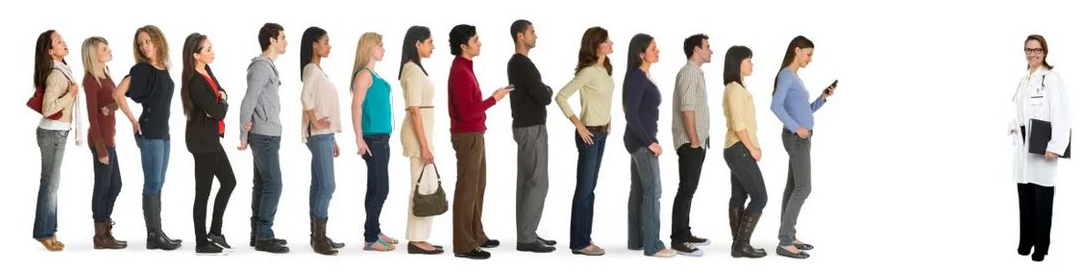
\includegraphics[width=0.9\textwidth]{figures/queue.png}}
\end{center}
\end{figure}
\begin{columns} 

    \begin{column}{.55\textwidth}       \vspace{-2ex}

\begin{table}[htbp]
% \caption{Stylized data structure. Here $k=A$ and $b=B$.}
\label{tab:data_structure}
\begin{threeparttable}
\tiny
\begin{tabular}{@{\extracolsep{-5pt}}l*{3}{c}}
\toprule
Obs & Selected  arm & Reward\\
\midrule
1 & A & 0  \\
2 & B & 0 \\
3 & A & 1 \\
4 & B & 0 \\
5 & A & 0 \\
6 & B & 1 \\
7 & A & 1 \\
8 & B & 0 \\
9 & A & 0 \\
10 & A & 1\\
11 & A & 1\\
12 & B & 0\\
13 & A & 1\\
14 & A & 0\\
15 & A & 1\\
16 & B & 0\\
%17 & ? & .\\
% \midrule
% OLS &  \multicolumn{7}{r}{$\widehat{\text{Reward}} = 0.6 - 0.433 \times \mathds{1}_{\text{arm B}}$}\\
% BOLS & \multicolumn{7}{r}{$ - 0.443 = \frac{0.5\times 1 + 0\times1+ \sqrt{\frac{1\times 3}{1+3}}\times 0.667+\sqrt{\frac{1\times 3}{1+3}}\times 0.667}{1+1+\sqrt{\frac{1\times 3}{1+3}}+\sqrt{\frac{1\times 3}{1+3}}}$}\\
%  &  \multicolumn{7}{r}{$\widehat{\text{Reward}} = 0.6 - 0.443 \times \mathds{1}_{\text{arm B}}$} \\
\bottomrule
\end{tabular}
% \begin{tablenotes}[para,flushleft]
%       {\textit{Note:} The table shows fictions data in a stylized structure for adaptive experiments. There are two arms A and B. The first batch is batch 0 where the arms would be randomly assigned. Afterwards treatment would be assigned according to one of the bandit algorithms (e.g. Thompson sampling).}
% \end{tablenotes}
\end{threeparttable}
\end{table}

\renewcommand{\baselinestretch}{1.45}
    \end{column}%
     \begin{column}{.5\textwidth}       \vspace{-2ex}

\begin{itemize}
    \item  Does arm A or arm B\\ perform better?\\[2ex]
    \item Which arm to play\\ in next trial (round 17)?
\end{itemize}
\end{column}
\end{columns}

\end{frame}




\begin{frame}\frametitle{Bandits $>>$ A/B Tests}
\renewcommand{\baselinestretch}{1}

\begin{itemize}
    \item Push to replace non-adaptive randomized trials with bandits
    \begin{itemize}
        \item In development and labor economics, finance, biostats, health, \ldots
        \item Can improve outcomes for participants (optimize regret)
        \item Can improve policies learned at the end of trial (best-arm identification)
    \end{itemize}
    \item \textbf{\textcolor{BrewerRed}{Problem}:}
    \begin{itemize}
        \item Bandits are not easy to implement\\
        Not available in statistical software like Stata
        \item Bandits break inference\\
        Adaptive arm allocations\\ $\rightarrow$ breaks asymptotics of usual estimators\\ $\rightarrow$ wrong confidence intervals
    \end{itemize}
    \item \textbf{{Solution}: Batched OLS (BOLS) for  \href{https://rostam-afschar.de/bbandits/bbandits.htm}{Batched Bandits}}
\end{itemize}

\end{frame}


\begin{frame}\frametitle{A Simple Example}
\renewcommand{\baselinestretch}{1}

\begin{itemize}
    \item OLS and BOLS under Beta-Bernoulli two-arm Thompson Sampling with batch size $N_t=100$ at batch $t =10$
    \item All simulations are with no margin ($\beta_1=\beta_0=0$)
\end{itemize}
\begin{figure}[h]
\begin{center}
% \caption{OLS and BOLS under Beta-Bernoulli two-arm Thompson Sampling with batch size $N_t=100$ at batch $t =10$}\label{OLS and BOLS under Beta-Bernoulli two-arm Thompson Sampling with batch size=100 at batch 10}
	\begin{subfigure}[t]{0.49\textwidth}
{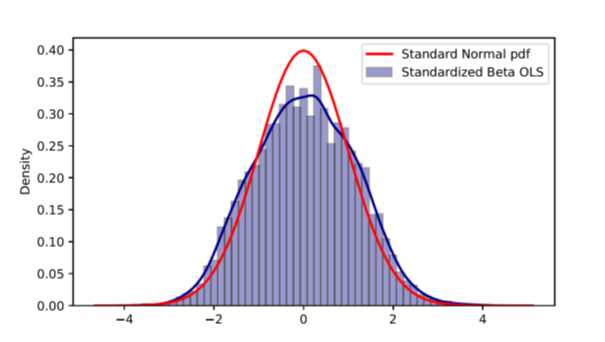
\includegraphics[width=1\textwidth]{figures/grafik3}}
           \caption{Empirical distribution of standard-\\\quad\; ized OLS estimator for the margin}
           \label{fig:Empirical distribution of standardized OLS estimator for the margin}	
  \end{subfigure}%
	\begin{subfigure}[t]{0.49\textwidth}
{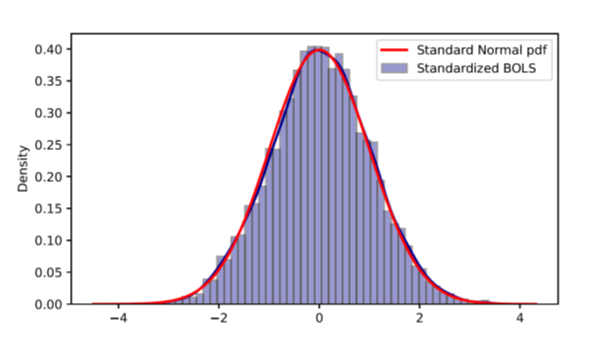
\includegraphics[width=1\textwidth]{figures/grafik4.png}}
           \caption{Empirical distribution of standard-\\\quad\; ized BOLS estimator for the margin}
           \label{fig:Empirical distribution of standardized BOLS estimator for the margin}	
  \end{subfigure}   
\end{center}
\vspace*{-4.5ex}
\end{figure}
\begin{center}
% \begin{minipage}{0.9\textwidth}
%     \footnotesize{
% 	\emph{Notes:}  All simulations are with no margin ($\beta_1=\beta_0=0$).}  
%     \end{minipage}
\end{center}

\end{frame}

\section{Batchwise Data Collection}
{
\setbeamercolor{background canvas}{bg=BrewerBlue}
\begin{frame}
\centering
\Huge
\textcolor{white}{Batchwise Data Collection}
\thispagestyle{empty}
\end{frame}
}



\begin{frame}\frametitle{Stylized data structure}
\renewcommand{\baselinestretch}{1}

\begin{table}[htbp]
\centering 

% \caption{Stylized data structure. Here $k=A$ and $b=B$.}
\label{tab:data_structure}
\begin{threeparttable}
\tiny
\begin{tabular}{@{\extracolsep{-5pt}}l*{3}{c}>{\columncolor{white!25}}{c}>{\columncolor{white!25}}{c}>{\columncolor{white!25}}{c}>{\columncolor{white!25}}{c}}
\toprule
Obs & Selected  arm & Batch & Reward & \color{white}{True Expected Reward} & \color{white}{OLS}& \color{white}{Batch-Wise OLS} & \color{white}{$\omega_t$}\\
\midrule
1 & A & 0 & . & \color{white}{0.5} & \color{white}{0.600} & \color{white}{0.500}& \color{white}{$\sqrt{\frac{2\times 2}{2+2}}$} \\
2 & B & 0 & . & \color{white}{0.2} & \color{white}{0.167} & \color{white}{0.000} &\color{white}{$\sqrt{\frac{2\times 2}{2+2}}$}\\
3 & A & 0 & . & \color{white}{0.5} & \color{white}{0.600} & \color{white}{0.500}&\color{white}{ $\sqrt{\frac{2\times 2}{2+2}}$}\\
4 & B & 0 & . & \color{white}{0.2} & \color{white}{0.167} & \color{white}{0.000}&\color{white}{ $\sqrt{\frac{2\times 2}{2+2}}$}\\
\rowcolor{blue1!20}
5 & . & 1 & . & \color{blue1!20}{0.5} & \color{blue1!20}{0.600} & \color{blue1!20}{0.500}&\color{blue1!20}{ $\sqrt{\frac{2\times 2}{2+2}}$}\\
\rowcolor{blue1!20}
6 & . & 1 & . & \color{blue1!20}{0.2} & \color{blue1!20}{0.167} & \color{blue1!20}{0.500}&\color{blue1!20}{ $\sqrt{\frac{2\times 2}{2+2}}$}\\
\rowcolor{blue1!20}
7 & . & 1 & . & \color{blue1!20}{0.5} &  \color{blue1!20}{0.600}& \color{blue1!20}{0.500}&\color{blue1!20}{ $\sqrt{\frac{2\times 2}{2+2}}$}\\
\rowcolor{blue1!20}
8 & . & 1 & . & \color{blue1!20}{0.2} &  \color{blue1!20}{0.167}& \color{blue1!20}{0.500}&\color{blue1!20}{ $\sqrt{\frac{2\times 2}{2+2}}$}\\
\rowcolor{blue1!40}
9 & . & 2 & . & \color{blue1!40}{0.5} & \color{blue1!40}{0.600} & \color{blue1!40}{0.667}&\color{blue1!40}{ $\sqrt{\frac{1\times 3}{1+3}}$}\\
\rowcolor{blue1!40}
10 & . & 2 & . & \color{blue1!40}{0.2} & \color{blue1!40}{0.600} & \color{blue1!40}{0.667}&\color{blue1!40}{$\sqrt{\frac{1\times 3}{1+3}}$}\\
\rowcolor{blue1!40}
11 & . & 2 & . & \color{blue1!40}{0.5} & \color{blue1!40}{0.600} & \color{blue1!40}{0.667}&\color{blue1!40}{$\sqrt{\frac{1\times 3}{1+3}}$}\\
\rowcolor{blue1!40}
12 & . & 2 & . & \color{blue1!40}{0.2} & \color{blue1!40}{0.167} & \color{blue1!40}{0.000}&\color{blue1!40}{$\sqrt{\frac{1\times 3}{1+3}}$}\\
\rowcolor{blue1!60}
13 & . & 3 & . & \color{blue1!60}{0.5} & \color{blue1!60}{0.600} & \color{blue1!60}{0.667}&\color{blue1!60}{$\sqrt{\frac{1\times 3}{1+3}}$}\\
\rowcolor{blue1!60}
14 & . & 3 & . & \color{blue1!60}{0.2} & \color{blue1!60}{0.600} & \color{blue1!60}{0.667}&\color{blue1!60}{$\sqrt{\frac{1\times 3}{1+3}}$}\\
\rowcolor{blue1!60}
15 & . & 3 & . & \color{blue1!60}{0.5} & \color{blue1!60}{0.600} & \color{blue1!60}{0.667}&\color{blue1!60}{$\sqrt{\frac{1\times 3}{1+3}}$}\\
\rowcolor{blue1!60}
16 & . & 3 & . & \color{blue1!60}{0.2} & \color{blue1!60}{0.167} & \color{blue1!60}{0.000}&\color{blue1!60}{$\sqrt{\frac{1\times 3}{1+3}}$}\\
% \midrule
% OLS &  \multicolumn{7}{r}{$\widehat{\text{Reward}} = 0.6 - 0.433 \times \mathds{1}_{\text{arm B}}$}\\
% BOLS & \multicolumn{7}{r}{$ - 0.443 = \frac{0.5\times 1 + 0\times1+ \sqrt{\frac{1\times 3}{1+3}}\times 0.667+\sqrt{\frac{1\times 3}{1+3}}\times 0.667}{1+1+\sqrt{\frac{1\times 3}{1+3}}+\sqrt{\frac{1\times 3}{1+3}}}$}\\
%  &  \multicolumn{7}{r}{$\widehat{\text{Reward}} = 0.6 - 0.443 \times \mathds{1}_{\text{arm B}}$} \\
\bottomrule
\end{tabular}
% \begin{tablenotes}[para,flushleft]
%       {\textit{Note:} The table shows fictions data in a stylized structure for adaptive experiments. There are two arms A and B. The first batch is batch 0 where the arms would be randomly assigned. Afterwards treatment would be assigned according to one of the bandit algorithms (e.g. Thompson sampling).}
% \end{tablenotes}
\end{threeparttable}
\end{table}

\renewcommand{\baselinestretch}{1.45}
\end{frame}





\begin{frame}\frametitle{Stylized data structure}
\renewcommand{\baselinestretch}{1}

\begin{table}[htbp]
\centering 

% \caption{Stylized data structure. Here $k=A$ and $b=B$.}
\label{tab:data_structure}
\begin{threeparttable}
\tiny
\begin{tabular}{@{\extracolsep{-5pt}}l*{3}{c}>{\columncolor{white!25}}{c}>{\columncolor{white!25}}{c}>{\columncolor{white!25}}{c}>{\columncolor{white!25}}{c}}
\toprule
Obs & Selected  arm & Batch & Reward & \color{white}{True Expected Reward} & \color{white}{OLS}& \color{white}{Batch-Wise OLS} & \color{white}{$\omega_t$}\\
\midrule
1 & A & 0 & 0 & \color{white}{0.5} & \color{white}{0.600} & \color{white}{0.500}& \color{white}{$\sqrt{\frac{2\times 2}{2+2}}$} \\
2 & B & 0 & 0 & \color{white}{0.2} & \color{white}{0.167} & \color{white}{0.000} &\color{white}{$\sqrt{\frac{2\times 2}{2+2}}$}\\
3 & A & 0 & 1 & \color{white}{0.5} & \color{white}{0.600} & \color{white}{0.500}&\color{white}{ $\sqrt{\frac{2\times 2}{2+2}}$}\\
4 & B & 0 & 0 & \color{white}{0.2} & \color{white}{0.167} & \color{white}{0.000}&\color{white}{ $\sqrt{\frac{2\times 2}{2+2}}$}\\
\rowcolor{blue1!20}
5 & . & 1 & . & \color{blue1!20}{0.5} & \color{blue1!20}{0.600} & \color{blue1!20}{0.500}&\color{blue1!20}{ $\sqrt{\frac{2\times 2}{2+2}}$}\\
\rowcolor{blue1!20}
6 & . & 1 & . & \color{blue1!20}{0.2} & \color{blue1!20}{0.167} & \color{blue1!20}{0.500}&\color{blue1!20}{ $\sqrt{\frac{2\times 2}{2+2}}$}\\
\rowcolor{blue1!20}
7 & . & 1 & . & \color{blue1!20}{0.5} &  \color{blue1!20}{0.600}& \color{blue1!20}{0.500}&\color{blue1!20}{ $\sqrt{\frac{2\times 2}{2+2}}$}\\
\rowcolor{blue1!20}
8 & . & 1 & . & \color{blue1!20}{0.2} &  \color{blue1!20}{0.167}& \color{blue1!20}{0.500}&\color{blue1!20}{ $\sqrt{\frac{2\times 2}{2+2}}$}\\
\rowcolor{blue1!40}
9 & . & 2 & . & \color{blue1!40}{0.5} & \color{blue1!40}{0.600} & \color{blue1!40}{0.667}&\color{blue1!40}{ $\sqrt{\frac{1\times 3}{1+3}}$}\\
\rowcolor{blue1!40}
10 & . & 2 & . & \color{blue1!40}{0.2} & \color{blue1!40}{0.600} & \color{blue1!40}{0.667}&\color{blue1!40}{$\sqrt{\frac{1\times 3}{1+3}}$}\\
\rowcolor{blue1!40}
11 & . & 2 & . & \color{blue1!40}{0.5} & \color{blue1!40}{0.600} & \color{blue1!40}{0.667}&\color{blue1!40}{$\sqrt{\frac{1\times 3}{1+3}}$}\\
\rowcolor{blue1!40}
12 & . & 2 & . & \color{blue1!40}{0.2} & \color{blue1!40}{0.167} & \color{blue1!40}{0.000}&\color{blue1!40}{$\sqrt{\frac{1\times 3}{1+3}}$}\\
\rowcolor{blue1!60}
13 & . & 3 & . & \color{blue1!60}{0.5} & \color{blue1!60}{0.600} & \color{blue1!60}{0.667}&\color{blue1!60}{$\sqrt{\frac{1\times 3}{1+3}}$}\\
\rowcolor{blue1!60}
14 & . & 3 & . & \color{blue1!60}{0.2} & \color{blue1!60}{0.600} & \color{blue1!60}{0.667}&\color{blue1!60}{$\sqrt{\frac{1\times 3}{1+3}}$}\\
\rowcolor{blue1!60}
15 & . & 3 & . & \color{blue1!60}{0.5} & \color{blue1!60}{0.600} & \color{blue1!60}{0.667}&\color{blue1!60}{$\sqrt{\frac{1\times 3}{1+3}}$}\\
\rowcolor{blue1!60}
16 & . & 3 & . & \color{blue1!60}{0.2} & \color{blue1!60}{0.167} & \color{blue1!60}{0.000}&\color{blue1!60}{$\sqrt{\frac{1\times 3}{1+3}}$}\\
% \midrule
% OLS &  \multicolumn{7}{r}{$\widehat{\text{Reward}} = 0.6 - 0.433 \times \mathds{1}_{\text{arm B}}$}\\
% BOLS & \multicolumn{7}{r}{$ - 0.443 = \frac{0.5\times 1 + 0\times1+ \sqrt{\frac{1\times 3}{1+3}}\times 0.667+\sqrt{\frac{1\times 3}{1+3}}\times 0.667}{1+1+\sqrt{\frac{1\times 3}{1+3}}+\sqrt{\frac{1\times 3}{1+3}}}$}\\
%  &  \multicolumn{7}{r}{$\widehat{\text{Reward}} = 0.6 - 0.443 \times \mathds{1}_{\text{arm B}}$} \\
\bottomrule
\end{tabular}
% \begin{tablenotes}[para,flushleft]
%       {\textit{Note:} The table shows fictions data in a stylized structure for adaptive experiments. There are two arms A and B. The first batch is batch 0 where the arms would be randomly assigned. Afterwards treatment would be assigned according to one of the bandit algorithms (e.g. Thompson sampling).}
% \end{tablenotes}
\end{threeparttable}
\end{table}

\renewcommand{\baselinestretch}{1.45}
\end{frame}


\begin{frame}\frametitle{Stylized data structure}
\renewcommand{\baselinestretch}{1}

\begin{table}[htbp]
\centering 

% \caption{Stylized data structure. Here $k=A$ and $b=B$.}
\label{tab:data_structure}
\begin{threeparttable}
\tiny
\begin{tabular}{@{\extracolsep{-5pt}}l*{3}{c}>{\columncolor{white!25}}{c}>{\columncolor{white!25}}{c}>{\columncolor{white!25}}{c}>{\columncolor{white!25}}{c}}
\toprule
Obs & Selected  arm & Batch & Reward & \color{white}{True Expected Reward} & \color{white}{OLS}& \color{white}{Batch-Wise OLS} & \color{white}{$\omega_t$}\\
\midrule
1 & A & 0 & 0 & \color{white}{0.5} & \color{white}{0.600} & \color{white}{0.500}& \color{white}{$\sqrt{\frac{2\times 2}{2+2}}$} \\
2 & B & 0 & 0 & \color{white}{0.2} & \color{white}{0.167} & \color{white}{0.000} &\color{white}{$\sqrt{\frac{2\times 2}{2+2}}$}\\
3 & A & 0 & 1 & \color{white}{0.5} & \color{white}{0.600} & \color{white}{0.500}&\color{white}{ $\sqrt{\frac{2\times 2}{2+2}}$}\\
4 & B & 0 & 0 & \color{white}{0.2} & \color{white}{0.167} & \color{white}{0.000}&\color{white}{ $\sqrt{\frac{2\times 2}{2+2}}$}\\
\rowcolor{blue1!20}
5 & A & 1 & . & \color{blue1!20}{0.5} & \color{blue1!20}{0.600} & \color{blue1!20}{0.500}&\color{blue1!20}{ $\sqrt{\frac{2\times 2}{2+2}}$}\\
\rowcolor{blue1!20}
6 & B & 1 & . & \color{blue1!20}{0.2} & \color{blue1!20}{0.167} & \color{blue1!20}{0.500}&\color{blue1!20}{ $\sqrt{\frac{2\times 2}{2+2}}$}\\
\rowcolor{blue1!20}
7 & A & 1 & . & \color{blue1!20}{0.5} &  \color{blue1!20}{0.600}& \color{blue1!20}{0.500}&\color{blue1!20}{ $\sqrt{\frac{2\times 2}{2+2}}$}\\
\rowcolor{blue1!20}
8 & B & 1 & . & \color{blue1!20}{0.2} &  \color{blue1!20}{0.167}& \color{blue1!20}{0.500}&\color{blue1!20}{ $\sqrt{\frac{2\times 2}{2+2}}$}\\
\rowcolor{blue1!40}
9 & . & 2 & . & \color{blue1!40}{0.5} & \color{blue1!40}{0.600} & \color{blue1!40}{0.667}&\color{blue1!40}{ $\sqrt{\frac{1\times 3}{1+3}}$}\\
\rowcolor{blue1!40}
10 & . & 2 & . & \color{blue1!40}{0.2} & \color{blue1!40}{0.600} & \color{blue1!40}{0.667}&\color{blue1!40}{$\sqrt{\frac{1\times 3}{1+3}}$}\\
\rowcolor{blue1!40}
11 & . & 2 & . & \color{blue1!40}{0.5} & \color{blue1!40}{0.600} & \color{blue1!40}{0.667}&\color{blue1!40}{$\sqrt{\frac{1\times 3}{1+3}}$}\\
\rowcolor{blue1!40}
12 & . & 2 & . & \color{blue1!40}{0.2} & \color{blue1!40}{0.167} & \color{blue1!40}{0.000}&\color{blue1!40}{$\sqrt{\frac{1\times 3}{1+3}}$}\\
\rowcolor{blue1!60}
13 & . & 3 & . & \color{blue1!60}{0.5} & \color{blue1!60}{0.600} & \color{blue1!60}{0.667}&\color{blue1!60}{$\sqrt{\frac{1\times 3}{1+3}}$}\\
\rowcolor{blue1!60}
14 & . & 3 & . & \color{blue1!60}{0.2} & \color{blue1!60}{0.600} & \color{blue1!60}{0.667}&\color{blue1!60}{$\sqrt{\frac{1\times 3}{1+3}}$}\\
\rowcolor{blue1!60}
15 & . & 3 & . & \color{blue1!60}{0.5} & \color{blue1!60}{0.600} & \color{blue1!60}{0.667}&\color{blue1!60}{$\sqrt{\frac{1\times 3}{1+3}}$}\\
\rowcolor{blue1!60}
16 & . & 3 & . & \color{blue1!60}{0.2} & \color{blue1!60}{0.167} & \color{blue1!60}{0.000}&\color{blue1!60}{$\sqrt{\frac{1\times 3}{1+3}}$}\\
% \midrule
% OLS &  \multicolumn{7}{r}{$\widehat{\text{Reward}} = 0.6 - 0.433 \times \mathds{1}_{\text{arm B}}$}\\
% BOLS & \multicolumn{7}{r}{$ - 0.443 = \frac{0.5\times 1 + 0\times1+ \sqrt{\frac{1\times 3}{1+3}}\times 0.667+\sqrt{\frac{1\times 3}{1+3}}\times 0.667}{1+1+\sqrt{\frac{1\times 3}{1+3}}+\sqrt{\frac{1\times 3}{1+3}}}$}\\
%  &  \multicolumn{7}{r}{$\widehat{\text{Reward}} = 0.6 - 0.443 \times \mathds{1}_{\text{arm B}}$} \\
\bottomrule
\end{tabular}
% \begin{tablenotes}[para,flushleft]
%       {\textit{Note:} The table shows fictions data in a stylized structure for adaptive experiments. There are two arms A and B. The first batch is batch 0 where the arms would be randomly assigned. Afterwards treatment would be assigned according to one of the bandit algorithms (e.g. Thompson sampling).}
% \end{tablenotes}
\end{threeparttable}
\end{table}

\renewcommand{\baselinestretch}{1.45}
\end{frame}



\begin{frame}\frametitle{Stylized data structure}
\renewcommand{\baselinestretch}{1}

\begin{table}[htbp]
\centering 

% \caption{Stylized data structure. Here $k=A$ and $b=B$.}
\label{tab:data_structure}
\begin{threeparttable}
\tiny
\begin{tabular}{@{\extracolsep{-5pt}}l*{3}{c}>{\columncolor{white!25}}{c}>{\columncolor{white!25}}{c}>{\columncolor{white!25}}{c}>{\columncolor{white!25}}{c}}
\toprule
Obs & Selected  arm & Batch & Reward & \color{white}{True Expected Reward} & \color{white}{OLS}& \color{white}{Batch-Wise OLS} & \color{white}{$\omega_t$}\\
\midrule
1 & A & 0 & 0 & \color{white}{0.5} & \color{white}{0.600} & \color{white}{0.500}& \color{white}{$\sqrt{\frac{2\times 2}{2+2}}$} \\
2 & B & 0 & 0 & \color{white}{0.2} & \color{white}{0.167} & \color{white}{0.000} &\color{white}{$\sqrt{\frac{2\times 2}{2+2}}$}\\
3 & A & 0 & 1 & \color{white}{0.5} & \color{white}{0.600} & \color{white}{0.500}&\color{white}{ $\sqrt{\frac{2\times 2}{2+2}}$}\\
4 & B & 0 & 0 & \color{white}{0.2} & \color{white}{0.167} & \color{white}{0.000}&\color{white}{ $\sqrt{\frac{2\times 2}{2+2}}$}\\
\rowcolor{blue1!20}
5 & A & 1 & 0 & \color{blue1!20}{0.5} & \color{blue1!20}{0.600} & \color{blue1!20}{0.500}&\color{blue1!20}{ $\sqrt{\frac{2\times 2}{2+2}}$}\\
\rowcolor{blue1!20}
6 & B & 1 & 1 & \color{blue1!20}{0.2} & \color{blue1!20}{0.167} & \color{blue1!20}{0.500}&\color{blue1!20}{ $\sqrt{\frac{2\times 2}{2+2}}$}\\
\rowcolor{blue1!20}
7 & A & 1 & 1 & \color{blue1!20}{0.5} &  \color{blue1!20}{0.600}& \color{blue1!20}{0.500}&\color{blue1!20}{ $\sqrt{\frac{2\times 2}{2+2}}$}\\
\rowcolor{blue1!20}
8 & B & 1 & 0 & \color{blue1!20}{0.2} &  \color{blue1!20}{0.167}& \color{blue1!20}{0.500}&\color{blue1!20}{ $\sqrt{\frac{2\times 2}{2+2}}$}\\
\rowcolor{blue1!40}
9 & . & 2 & . & \color{blue1!40}{0.5} & \color{blue1!40}{0.600} & \color{blue1!40}{0.667}&\color{blue1!40}{ $\sqrt{\frac{1\times 3}{1+3}}$}\\
\rowcolor{blue1!40}
10 & . & 2 & . & \color{blue1!40}{0.2} & \color{blue1!40}{0.600} & \color{blue1!40}{0.667}&\color{blue1!40}{$\sqrt{\frac{1\times 3}{1+3}}$}\\
\rowcolor{blue1!40}
11 & . & 2 & . & \color{blue1!40}{0.5} & \color{blue1!40}{0.600} & \color{blue1!40}{0.667}&\color{blue1!40}{$\sqrt{\frac{1\times 3}{1+3}}$}\\
\rowcolor{blue1!40}
12 & . & 2 & . & \color{blue1!40}{0.2} & \color{blue1!40}{0.167} & \color{blue1!40}{0.000}&\color{blue1!40}{$\sqrt{\frac{1\times 3}{1+3}}$}\\
\rowcolor{blue1!60}
13 & . & 3 & . & \color{blue1!60}{0.5} & \color{blue1!60}{0.600} & \color{blue1!60}{0.667}&\color{blue1!60}{$\sqrt{\frac{1\times 3}{1+3}}$}\\
\rowcolor{blue1!60}
14 & . & 3 & . & \color{blue1!60}{0.2} & \color{blue1!60}{0.600} & \color{blue1!60}{0.667}&\color{blue1!60}{$\sqrt{\frac{1\times 3}{1+3}}$}\\
\rowcolor{blue1!60}
15 & . & 3 & . & \color{blue1!60}{0.5} & \color{blue1!60}{0.600} & \color{blue1!60}{0.667}&\color{blue1!60}{$\sqrt{\frac{1\times 3}{1+3}}$}\\
\rowcolor{blue1!60}
16 & . & 3 & . & \color{blue1!60}{0.2} & \color{blue1!60}{0.167} & \color{blue1!60}{0.000}&\color{blue1!60}{$\sqrt{\frac{1\times 3}{1+3}}$}\\
% \midrule
% OLS &  \multicolumn{7}{r}{$\widehat{\text{Reward}} = 0.6 - 0.433 \times \mathds{1}_{\text{arm B}}$}\\
% BOLS & \multicolumn{7}{r}{$ - 0.443 = \frac{0.5\times 1 + 0\times1+ \sqrt{\frac{1\times 3}{1+3}}\times 0.667+\sqrt{\frac{1\times 3}{1+3}}\times 0.667}{1+1+\sqrt{\frac{1\times 3}{1+3}}+\sqrt{\frac{1\times 3}{1+3}}}$}\\
%  &  \multicolumn{7}{r}{$\widehat{\text{Reward}} = 0.6 - 0.443 \times \mathds{1}_{\text{arm B}}$} \\
\bottomrule
\end{tabular}
% \begin{tablenotes}[para,flushleft]
%       {\textit{Note:} The table shows fictions data in a stylized structure for adaptive experiments. There are two arms A and B. The first batch is batch 0 where the arms would be randomly assigned. Afterwards treatment would be assigned according to one of the bandit algorithms (e.g. Thompson sampling).}
% \end{tablenotes}
\end{threeparttable}
\end{table}

\renewcommand{\baselinestretch}{1.45}
\end{frame}



\begin{frame}\frametitle{Stylized data structure}
\renewcommand{\baselinestretch}{1}

\begin{table}[htbp]
\centering 

% \caption{Stylized data structure. Here $k=A$ and $b=B$.}
\label{tab:data_structure}
\begin{threeparttable}
\tiny
\begin{tabular}{@{\extracolsep{-5pt}}l*{3}{c}>{\columncolor{white!25}}{c}>{\columncolor{white!25}}{c}>{\columncolor{white!25}}{c}>{\columncolor{white!25}}{c}}
\toprule
Obs & Selected  arm & Batch & Reward & \color{white}{True Expected Reward} & \color{white}{OLS}& \color{white}{Batch-Wise OLS} & \color{white}{$\omega_t$}\\
\midrule
1 & A & 0 & 0 & \color{white}{0.5} & \color{white}{0.600} & \color{white}{0.500}& \color{white}{$\sqrt{\frac{2\times 2}{2+2}}$} \\
2 & B & 0 & 0 & \color{white}{0.2} & \color{white}{0.167} & \color{white}{0.000} &\color{white}{$\sqrt{\frac{2\times 2}{2+2}}$}\\
3 & A & 0 & 1 & \color{white}{0.5} & \color{white}{0.600} & \color{white}{0.500}&\color{white}{ $\sqrt{\frac{2\times 2}{2+2}}$}\\
4 & B & 0 & 0 & \color{white}{0.2} & \color{white}{0.167} & \color{white}{0.000}&\color{white}{ $\sqrt{\frac{2\times 2}{2+2}}$}\\
\rowcolor{blue1!20}
5 & A & 1 & 0 & \color{blue1!20}{0.5} & \color{blue1!20}{0.600} & \color{blue1!20}{0.500}&\color{blue1!20}{ $\sqrt{\frac{2\times 2}{2+2}}$}\\
\rowcolor{blue1!20}
6 & B & 1 & 1 & \color{blue1!20}{0.2} & \color{blue1!20}{0.167} & \color{blue1!20}{0.500}&\color{blue1!20}{ $\sqrt{\frac{2\times 2}{2+2}}$}\\
\rowcolor{blue1!20}
7 & A & 1 & 1 & \color{blue1!20}{0.5} &  \color{blue1!20}{0.600}& \color{blue1!20}{0.500}&\color{blue1!20}{ $\sqrt{\frac{2\times 2}{2+2}}$}\\
\rowcolor{blue1!20}
8 & B & 1 & 0 & \color{blue1!20}{0.2} &  \color{blue1!20}{0.167}& \color{blue1!20}{0.500}&\color{blue1!20}{ $\sqrt{\frac{2\times 2}{2+2}}$}\\
\rowcolor{blue1!40}
9 & A & 2 & . & \color{blue1!40}{0.5} & \color{blue1!40}{0.600} & \color{blue1!40}{0.667}&\color{blue1!40}{ $\sqrt{\frac{1\times 3}{1+3}}$}\\
\rowcolor{blue1!40}
10 & A & 2 & . & \color{blue1!40}{0.2} & \color{blue1!40}{0.600} & \color{blue1!40}{0.667}&\color{blue1!40}{$\sqrt{\frac{1\times 3}{1+3}}$}\\
\rowcolor{blue1!40}
11 & A & 2 & . & \color{blue1!40}{0.5} & \color{blue1!40}{0.600} & \color{blue1!40}{0.667}&\color{blue1!40}{$\sqrt{\frac{1\times 3}{1+3}}$}\\
\rowcolor{blue1!40}
12 & B & 2 & . & \color{blue1!40}{0.2} & \color{blue1!40}{0.167} & \color{blue1!40}{0.000}&\color{blue1!40}{$\sqrt{\frac{1\times 3}{1+3}}$}\\
\rowcolor{blue1!60}
13 & . & 3 & . & \color{blue1!60}{0.5} & \color{blue1!60}{0.600} & \color{blue1!60}{0.667}&\color{blue1!60}{$\sqrt{\frac{1\times 3}{1+3}}$}\\
\rowcolor{blue1!60}
14 & . & 3 & . & \color{blue1!60}{0.2} & \color{blue1!60}{0.600} & \color{blue1!60}{0.667}&\color{blue1!60}{$\sqrt{\frac{1\times 3}{1+3}}$}\\
\rowcolor{blue1!60}
15 & . & 3 & . & \color{blue1!60}{0.5} & \color{blue1!60}{0.600} & \color{blue1!60}{0.667}&\color{blue1!60}{$\sqrt{\frac{1\times 3}{1+3}}$}\\
\rowcolor{blue1!60}
16 & . & 3 & . & \color{blue1!60}{0.2} & \color{blue1!60}{0.167} & \color{blue1!60}{0.000}&\color{blue1!60}{$\sqrt{\frac{1\times 3}{1+3}}$}\\
% \midrule
% OLS &  \multicolumn{7}{r}{$\widehat{\text{Reward}} = 0.6 - 0.433 \times \mathds{1}_{\text{arm B}}$}\\
% BOLS & \multicolumn{7}{r}{$ - 0.443 = \frac{0.5\times 1 + 0\times1+ \sqrt{\frac{1\times 3}{1+3}}\times 0.667+\sqrt{\frac{1\times 3}{1+3}}\times 0.667}{1+1+\sqrt{\frac{1\times 3}{1+3}}+\sqrt{\frac{1\times 3}{1+3}}}$}\\
%  &  \multicolumn{7}{r}{$\widehat{\text{Reward}} = 0.6 - 0.443 \times \mathds{1}_{\text{arm B}}$} \\
\bottomrule
\end{tabular}
% \begin{tablenotes}[para,flushleft]
%       {\textit{Note:} The table shows fictions data in a stylized structure for adaptive experiments. There are two arms A and B. The first batch is batch 0 where the arms would be randomly assigned. Afterwards treatment would be assigned according to one of the bandit algorithms (e.g. Thompson sampling).}
% \end{tablenotes}
\end{threeparttable}
\end{table}

\renewcommand{\baselinestretch}{1.45}
\end{frame}


\begin{frame}\frametitle{Stylized data structure}
\renewcommand{\baselinestretch}{1}

\begin{table}[htbp]
\centering 

% \caption{Stylized data structure. Here $k=A$ and $b=B$.}
\label{tab:data_structure}
\begin{threeparttable}
\tiny
\begin{tabular}{@{\extracolsep{-5pt}}l*{3}{c}>{\columncolor{white!25}}{c}>{\columncolor{white!25}}{c}>{\columncolor{white!25}}{c}>{\columncolor{white!25}}{c}}
\toprule
Obs & Selected  arm & Batch & Reward & \color{white}{True Expected Reward} & \color{white}{OLS}& \color{white}{Batch-Wise OLS} & \color{white}{$\omega_t$}\\
\midrule
1 & A & 0 & 0 & \color{white}{0.5} & \color{white}{0.600} & \color{white}{0.500}& \color{white}{$\sqrt{\frac{2\times 2}{2+2}}$} \\
2 & B & 0 & 0 & \color{white}{0.2} & \color{white}{0.167} & \color{white}{0.000} &\color{white}{$\sqrt{\frac{2\times 2}{2+2}}$}\\
3 & A & 0 & 1 & \color{white}{0.5} & \color{white}{0.600} & \color{white}{0.500}&\color{white}{ $\sqrt{\frac{2\times 2}{2+2}}$}\\
4 & B & 0 & 0 & \color{white}{0.2} & \color{white}{0.167} & \color{white}{0.000}&\color{white}{ $\sqrt{\frac{2\times 2}{2+2}}$}\\
\rowcolor{blue1!20}
5 & A & 1 & 0 & \color{blue1!20}{0.5} & \color{blue1!20}{0.600} & \color{blue1!20}{0.500}&\color{blue1!20}{ $\sqrt{\frac{2\times 2}{2+2}}$}\\
\rowcolor{blue1!20}
6 & B & 1 & 1 & \color{blue1!20}{0.2} & \color{blue1!20}{0.167} & \color{blue1!20}{0.500}&\color{blue1!20}{ $\sqrt{\frac{2\times 2}{2+2}}$}\\
\rowcolor{blue1!20}
7 & A & 1 & 1 & \color{blue1!20}{0.5} &  \color{blue1!20}{0.600}& \color{blue1!20}{0.500}&\color{blue1!20}{ $\sqrt{\frac{2\times 2}{2+2}}$}\\
\rowcolor{blue1!20}
8 & B & 1 & 0 & \color{blue1!20}{0.2} &  \color{blue1!20}{0.167}& \color{blue1!20}{0.500}&\color{blue1!20}{ $\sqrt{\frac{2\times 2}{2+2}}$}\\
\rowcolor{blue1!40}
9 & A & 2 & 0 & \color{blue1!40}{0.5} & \color{blue1!40}{0.600} & \color{blue1!40}{0.667}&\color{blue1!40}{ $\sqrt{\frac{1\times 3}{1+3}}$}\\
\rowcolor{blue1!40}
10 & A & 2 & 1 & \color{blue1!40}{0.2} & \color{blue1!40}{0.600} & \color{blue1!40}{0.667}&\color{blue1!40}{$\sqrt{\frac{1\times 3}{1+3}}$}\\
\rowcolor{blue1!40}
11 & A & 2 & 1 & \color{blue1!40}{0.5} & \color{blue1!40}{0.600} & \color{blue1!40}{0.667}&\color{blue1!40}{$\sqrt{\frac{1\times 3}{1+3}}$}\\
\rowcolor{blue1!40}
12 & B & 2 & 0 & \color{blue1!40}{0.2} & \color{blue1!40}{0.167} & \color{blue1!40}{0.000}&\color{blue1!40}{$\sqrt{\frac{1\times 3}{1+3}}$}\\
\rowcolor{blue1!60}
13 & . & 3 & . & \color{blue1!60}{0.5} & \color{blue1!60}{0.600} & \color{blue1!60}{0.667}&\color{blue1!60}{$\sqrt{\frac{1\times 3}{1+3}}$}\\
\rowcolor{blue1!60}
14 & . & 3 & . & \color{blue1!60}{0.2} & \color{blue1!60}{0.600} & \color{blue1!60}{0.667}&\color{blue1!60}{$\sqrt{\frac{1\times 3}{1+3}}$}\\
\rowcolor{blue1!60}
15 & . & 3 & . & \color{blue1!60}{0.5} & \color{blue1!60}{0.600} & \color{blue1!60}{0.667}&\color{blue1!60}{$\sqrt{\frac{1\times 3}{1+3}}$}\\
\rowcolor{blue1!60}
16 & . & 3 & . & \color{blue1!60}{0.2} & \color{blue1!60}{0.167} & \color{blue1!60}{0.000}&\color{blue1!60}{$\sqrt{\frac{1\times 3}{1+3}}$}\\
% \midrule
% OLS &  \multicolumn{7}{r}{$\widehat{\text{Reward}} = 0.6 - 0.433 \times \mathds{1}_{\text{arm B}}$}\\
% BOLS & \multicolumn{7}{r}{$ - 0.443 = \frac{0.5\times 1 + 0\times1+ \sqrt{\frac{1\times 3}{1+3}}\times 0.667+\sqrt{\frac{1\times 3}{1+3}}\times 0.667}{1+1+\sqrt{\frac{1\times 3}{1+3}}+\sqrt{\frac{1\times 3}{1+3}}}$}\\
%  &  \multicolumn{7}{r}{$\widehat{\text{Reward}} = 0.6 - 0.443 \times \mathds{1}_{\text{arm B}}$} \\
\bottomrule
\end{tabular}
% \begin{tablenotes}[para,flushleft]
%       {\textit{Note:} The table shows fictions data in a stylized structure for adaptive experiments. There are two arms A and B. The first batch is batch 0 where the arms would be randomly assigned. Afterwards treatment would be assigned according to one of the bandit algorithms (e.g. Thompson sampling).}
% \end{tablenotes}
\end{threeparttable}
\end{table}

\renewcommand{\baselinestretch}{1.45}
\end{frame}


\begin{frame}\frametitle{Stylized data structure}
\renewcommand{\baselinestretch}{1}

\begin{table}[htbp]
\centering 

% \caption{Stylized data structure. Here $k=A$ and $b=B$.}
\label{tab:data_structure}
\begin{threeparttable}
\tiny
\begin{tabular}{@{\extracolsep{-5pt}}l*{3}{c}>{\columncolor{white!25}}{c}>{\columncolor{white!25}}{c}>{\columncolor{white!25}}{c}>{\columncolor{white!25}}{c}}
\toprule
Obs & Selected  arm & Batch & Reward & \color{white}{True Expected Reward} & \color{white}{OLS}& \color{white}{Batch-Wise OLS} & \color{white}{$\omega_t$}\\
\midrule
1 & A & 0 & 0 & \color{white}{0.5} & \color{white}{0.600} & \color{white}{0.500}& \color{white}{$\sqrt{\frac{2\times 2}{2+2}}$} \\
2 & B & 0 & 0 & \color{white}{0.2} & \color{white}{0.167} & \color{white}{0.000} &\color{white}{$\sqrt{\frac{2\times 2}{2+2}}$}\\
3 & A & 0 & 1 & \color{white}{0.5} & \color{white}{0.600} & \color{white}{0.500}&\color{white}{ $\sqrt{\frac{2\times 2}{2+2}}$}\\
4 & B & 0 & 0 & \color{white}{0.2} & \color{white}{0.167} & \color{white}{0.000}&\color{white}{ $\sqrt{\frac{2\times 2}{2+2}}$}\\
\rowcolor{blue1!20}
5 & A & 1 & 0 & \color{blue1!20}{0.5} & \color{blue1!20}{0.600} & \color{blue1!20}{0.500}&\color{blue1!20}{ $\sqrt{\frac{2\times 2}{2+2}}$}\\
\rowcolor{blue1!20}
6 & B & 1 & 1 & \color{blue1!20}{0.2} & \color{blue1!20}{0.167} & \color{blue1!20}{0.500}&\color{blue1!20}{ $\sqrt{\frac{2\times 2}{2+2}}$}\\
\rowcolor{blue1!20}
7 & A & 1 & 1 & \color{blue1!20}{0.5} &  \color{blue1!20}{0.600}& \color{blue1!20}{0.500}&\color{blue1!20}{ $\sqrt{\frac{2\times 2}{2+2}}$}\\
\rowcolor{blue1!20}
8 & B & 1 & 0 & \color{blue1!20}{0.2} &  \color{blue1!20}{0.167}& \color{blue1!20}{0.500}&\color{blue1!20}{ $\sqrt{\frac{2\times 2}{2+2}}$}\\
\rowcolor{blue1!40}
9 & A & 2 & 0 & \color{blue1!40}{0.5} & \color{blue1!40}{0.600} & \color{blue1!40}{0.667}&\color{blue1!40}{ $\sqrt{\frac{1\times 3}{1+3}}$}\\
\rowcolor{blue1!40}
10 & A & 2 & 1 & \color{blue1!40}{0.2} & \color{blue1!40}{0.600} & \color{blue1!40}{0.667}&\color{blue1!40}{$\sqrt{\frac{1\times 3}{1+3}}$}\\
\rowcolor{blue1!40}
11 & A & 2 & 1 & \color{blue1!40}{0.5} & \color{blue1!40}{0.600} & \color{blue1!40}{0.667}&\color{blue1!40}{$\sqrt{\frac{1\times 3}{1+3}}$}\\
\rowcolor{blue1!40}
12 & B & 2 & 0 & \color{blue1!40}{0.2} & \color{blue1!40}{0.167} & \color{blue1!40}{0.000}&\color{blue1!40}{$\sqrt{\frac{1\times 3}{1+3}}$}\\
\rowcolor{blue1!60}
13 & A & 3 & . & \color{blue1!60}{0.5} & \color{blue1!60}{0.600} & \color{blue1!60}{0.667}&\color{blue1!60}{$\sqrt{\frac{1\times 3}{1+3}}$}\\
\rowcolor{blue1!60}
14 & A & 3 & . & \color{blue1!60}{0.2} & \color{blue1!60}{0.600} & \color{blue1!60}{0.667}&\color{blue1!60}{$\sqrt{\frac{1\times 3}{1+3}}$}\\
\rowcolor{blue1!60}
15 & A & 3 & . & \color{blue1!60}{0.5} & \color{blue1!60}{0.600} & \color{blue1!60}{0.667}&\color{blue1!60}{$\sqrt{\frac{1\times 3}{1+3}}$}\\
\rowcolor{blue1!60}
16 & B & 3 & . & \color{blue1!60}{0.2} & \color{blue1!60}{0.167} & \color{blue1!60}{0.000}&\color{blue1!60}{$\sqrt{\frac{1\times 3}{1+3}}$}\\
% \midrule
% OLS &  \multicolumn{7}{r}{$\widehat{\text{Reward}} = 0.6 - 0.433 \times \mathds{1}_{\text{arm B}}$}\\
% BOLS & \multicolumn{7}{r}{$ - 0.443 = \frac{0.5\times 1 + 0\times1+ \sqrt{\frac{1\times 3}{1+3}}\times 0.667+\sqrt{\frac{1\times 3}{1+3}}\times 0.667}{1+1+\sqrt{\frac{1\times 3}{1+3}}+\sqrt{\frac{1\times 3}{1+3}}}$}\\
%  &  \multicolumn{7}{r}{$\widehat{\text{Reward}} = 0.6 - 0.443 \times \mathds{1}_{\text{arm B}}$} \\
\bottomrule
\end{tabular}
% \begin{tablenotes}[para,flushleft]
%       {\textit{Note:} The table shows fictions data in a stylized structure for adaptive experiments. There are two arms A and B. The first batch is batch 0 where the arms would be randomly assigned. Afterwards treatment would be assigned according to one of the bandit algorithms (e.g. Thompson sampling).}
% \end{tablenotes}
\end{threeparttable}
\end{table}

\renewcommand{\baselinestretch}{1.45}
\end{frame}



\begin{frame}\frametitle{Stylized data structure}
\renewcommand{\baselinestretch}{1}

\begin{table}[htbp]
\centering 

% \caption{Stylized data structure. Here $k=A$ and $b=B$.}
\label{tab:data_structure}
\begin{threeparttable}
\tiny
\begin{tabular}{@{\extracolsep{-5pt}}l*{3}{c}>{\columncolor{white!25}}{c}>{\columncolor{white!25}}{c}>{\columncolor{white!25}}{c}>{\columncolor{white!25}}{c}}
\toprule
Obs & Selected  arm & Batch & Reward & \color{white}{True Expected Reward} & \color{white}{OLS}& \color{white}{Batch-Wise OLS} & \color{white}{$\omega_t$}\\
\midrule
1 & A & 0 & 0 & \color{white}{0.5} & \color{white}{0.600} & \color{white}{0.500}& \color{white}{$\sqrt{\frac{2\times 2}{2+2}}$} \\
2 & B & 0 & 0 & \color{white}{0.2} & \color{white}{0.167} & \color{white}{0.000} &\color{white}{$\sqrt{\frac{2\times 2}{2+2}}$}\\
3 & A & 0 & 1 & \color{white}{0.5} & \color{white}{0.600} & \color{white}{0.500}&\color{white}{ $\sqrt{\frac{2\times 2}{2+2}}$}\\
4 & B & 0 & 0 & \color{white}{0.2} & \color{white}{0.167} & \color{white}{0.000}&\color{white}{ $\sqrt{\frac{2\times 2}{2+2}}$}\\
\rowcolor{blue1!20}
5 & A & 1 & 0 & \color{blue1!20}{0.5} & \color{blue1!20}{0.600} & \color{blue1!20}{0.500}&\color{blue1!20}{ $\sqrt{\frac{2\times 2}{2+2}}$}\\
\rowcolor{blue1!20}
6 & B & 1 & 1 & \color{blue1!20}{0.2} & \color{blue1!20}{0.167} & \color{blue1!20}{0.500}&\color{blue1!20}{ $\sqrt{\frac{2\times 2}{2+2}}$}\\
\rowcolor{blue1!20}
7 & A & 1 & 1 & \color{blue1!20}{0.5} &  \color{blue1!20}{0.600}& \color{blue1!20}{0.500}&\color{blue1!20}{ $\sqrt{\frac{2\times 2}{2+2}}$}\\
\rowcolor{blue1!20}
8 & B & 1 & 0 & \color{blue1!20}{0.2} &  \color{blue1!20}{0.167}& \color{blue1!20}{0.500}&\color{blue1!20}{ $\sqrt{\frac{2\times 2}{2+2}}$}\\
\rowcolor{blue1!40}
9 & A & 2 & 0 & \color{blue1!40}{0.5} & \color{blue1!40}{0.600} & \color{blue1!40}{0.667}&\color{blue1!40}{ $\sqrt{\frac{1\times 3}{1+3}}$}\\
\rowcolor{blue1!40}
10 & A & 2 & 1 & \color{blue1!40}{0.2} & \color{blue1!40}{0.600} & \color{blue1!40}{0.667}&\color{blue1!40}{$\sqrt{\frac{1\times 3}{1+3}}$}\\
\rowcolor{blue1!40}
11 & A & 2 & 1 & \color{blue1!40}{0.5} & \color{blue1!40}{0.600} & \color{blue1!40}{0.667}&\color{blue1!40}{$\sqrt{\frac{1\times 3}{1+3}}$}\\
\rowcolor{blue1!40}
12 & B & 2 & 0 & \color{blue1!40}{0.2} & \color{blue1!40}{0.167} & \color{blue1!40}{0.000}&\color{blue1!40}{$\sqrt{\frac{1\times 3}{1+3}}$}\\
\rowcolor{blue1!60}
13 & A & 3 & 1 & \color{blue1!60}{0.5} & \color{blue1!60}{0.600} & \color{blue1!60}{0.667}&\color{blue1!60}{$\sqrt{\frac{1\times 3}{1+3}}$}\\
\rowcolor{blue1!60}
14 & A & 3 & 0 & \color{blue1!60}{0.2} & \color{blue1!60}{0.600} & \color{blue1!60}{0.667}&\color{blue1!60}{$\sqrt{\frac{1\times 3}{1+3}}$}\\
\rowcolor{blue1!60}
15 & A & 3 & 1 & \color{blue1!60}{0.5} & \color{blue1!60}{0.600} & \color{blue1!60}{0.667}&\color{blue1!60}{$\sqrt{\frac{1\times 3}{1+3}}$}\\
\rowcolor{blue1!60}
16 & B & 3 & 0 & \color{blue1!60}{0.2} & \color{blue1!60}{0.167} & \color{blue1!60}{0.000}&\color{blue1!60}{$\sqrt{\frac{1\times 3}{1+3}}$}\\
% \midrule
% OLS &  \multicolumn{7}{r}{$\widehat{\text{Reward}} = 0.6 - 0.433 \times \mathds{1}_{\text{arm B}}$}\\
% BOLS & \multicolumn{7}{r}{$ - 0.443 = \frac{0.5\times 1 + 0\times1+ \sqrt{\frac{1\times 3}{1+3}}\times 0.667+\sqrt{\frac{1\times 3}{1+3}}\times 0.667}{1+1+\sqrt{\frac{1\times 3}{1+3}}+\sqrt{\frac{1\times 3}{1+3}}}$}\\
%  &  \multicolumn{7}{r}{$\widehat{\text{Reward}} = 0.6 - 0.443 \times \mathds{1}_{\text{arm B}}$} \\
\bottomrule
\end{tabular}
% \begin{tablenotes}[para,flushleft]
%       {\textit{Note:} The table shows fictions data in a stylized structure for adaptive experiments. There are two arms A and B. The first batch is batch 0 where the arms would be randomly assigned. Afterwards treatment would be assigned according to one of the bandit algorithms (e.g. Thompson sampling).}
% \end{tablenotes}
\end{threeparttable}
\end{table}

\renewcommand{\baselinestretch}{1.45}
\end{frame}


\begin{frame}\frametitle{Stylized data structure}
\renewcommand{\baselinestretch}{1}

\begin{table}[htbp]
\centering 

% \caption{Stylized data structure. Here $k=A$ and $b=B$.}
\label{tab:data_structure}
\begin{threeparttable}
\tiny
\begin{tabular}{@{\extracolsep{-5pt}}l*{3}{c}>{\columncolor{white!25}}{c}>{\columncolor{white!25}}{c}>{\columncolor{white!25}}{c}>{\columncolor{white!25}}{c}}
\toprule
Obs & Selected  arm & Batch & Reward & \color{black}{True Expected Reward} & \color{white}{OLS}& \color{white}{Batch-Wise OLS} & \color{white}{$\omega_t$}\\
\midrule
1 & A & 0 & 0 & \color{black}{0.5} & \color{white}{0.600} & \color{white}{0.500}& \color{white}{$\sqrt{\frac{2\times 2}{2+2}}$} \\
2 & B & 0 & 0 & \color{black}{0.2} & \color{white}{0.167} & \color{white}{0.000} &\color{white}{$\sqrt{\frac{2\times 2}{2+2}}$}\\
3 & A & 0 & 1 & \color{black}{0.5} & \color{white}{0.600} & \color{white}{0.500}&\color{white}{ $\sqrt{\frac{2\times 2}{2+2}}$}\\
4 & B & 0 & 0 & \color{black}{0.2} & \color{white}{0.167} & \color{white}{0.000}&\color{white}{ $\sqrt{\frac{2\times 2}{2+2}}$}\\
\rowcolor{blue1!20}
5 & A & 1 & 0 & \color{black}{0.5} & \color{blue1!20}{0.600} & \color{blue1!20}{0.500}&\color{blue1!20}{ $\sqrt{\frac{2\times 2}{2+2}}$}\\
\rowcolor{blue1!20}
6 & B & 1 & 1 & \color{black}{0.2} & \color{blue1!20}{0.167} & \color{blue1!20}{0.500}&\color{blue1!20}{ $\sqrt{\frac{2\times 2}{2+2}}$}\\
\rowcolor{blue1!20}
7 & A & 1 & 1 & \color{black}{0.5} &  \color{blue1!20}{0.600}& \color{blue1!20}{0.500}&\color{blue1!20}{ $\sqrt{\frac{2\times 2}{2+2}}$}\\
\rowcolor{blue1!20}
8 & B & 1 & 0 & \color{black}{0.2} &  \color{blue1!20}{0.167}& \color{blue1!20}{0.500}&\color{blue1!20}{ $\sqrt{\frac{2\times 2}{2+2}}$}\\
\rowcolor{blue1!40}
9 & A & 2 & 0 & \color{black}{0.5} & \color{blue1!40}{0.600} & \color{blue1!40}{0.667}&\color{blue1!40}{ $\sqrt{\frac{1\times 3}{1+3}}$}\\
\rowcolor{blue1!40}
10 & A & 2 & 1 & \color{black}{0.2} & \color{blue1!40}{0.600} & \color{blue1!40}{0.667}&\color{blue1!40}{$\sqrt{\frac{1\times 3}{1+3}}$}\\
\rowcolor{blue1!40}
11 & A & 2 & 1 & \color{black}{0.5} & \color{blue1!40}{0.600} & \color{blue1!40}{0.667}&\color{blue1!40}{$\sqrt{\frac{1\times 3}{1+3}}$}\\
\rowcolor{blue1!40}
12 & B & 2 & 0 & \color{black}{0.2} & \color{blue1!40}{0.167} & \color{blue1!40}{0.000}&\color{blue1!40}{$\sqrt{\frac{1\times 3}{1+3}}$}\\
\rowcolor{blue1!60}
13 & A & 3 & 1 & \color{black}{0.5} & \color{blue1!60}{0.600} & \color{blue1!60}{0.667}&\color{blue1!60}{$\sqrt{\frac{1\times 3}{1+3}}$}\\
\rowcolor{blue1!60}
14 & A & 3 & 0 & \color{black}{0.2} & \color{blue1!60}{0.600} & \color{blue1!60}{0.667}&\color{blue1!60}{$\sqrt{\frac{1\times 3}{1+3}}$}\\
\rowcolor{blue1!60}
15 & A & 3 & 1 & \color{black}{0.5} & \color{blue1!60}{0.600} & \color{blue1!60}{0.667}&\color{blue1!60}{$\sqrt{\frac{1\times 3}{1+3}}$}\\
\rowcolor{blue1!60}
16 & B & 3 & 0 & \color{black}{0.2} & \color{blue1!60}{0.167} & \color{blue1!60}{0.000}&\color{blue1!60}{$\sqrt{\frac{1\times 3}{1+3}}$}\\
% \midrule
% OLS &  \multicolumn{7}{r}{$\widehat{\text{Reward}} = 0.6 - 0.433 \times \mathds{1}_{\text{arm B}}$}\\
% BOLS & \multicolumn{7}{r}{$ - 0.443 = \frac{0.5\times 1 + 0\times1+ \sqrt{\frac{1\times 3}{1+3}}\times 0.667+\sqrt{\frac{1\times 3}{1+3}}\times 0.667}{1+1+\sqrt{\frac{1\times 3}{1+3}}+\sqrt{\frac{1\times 3}{1+3}}}$}\\
%  &  \multicolumn{7}{r}{$\widehat{\text{Reward}} = 0.6 - 0.443 \times \mathds{1}_{\text{arm B}}$} \\
\bottomrule
\end{tabular}
% \begin{tablenotes}[para,flushleft]
%       {\textit{Note:} The table shows fictions data in a stylized structure for adaptive experiments. There are two arms A and B. The first batch is batch 0 where the arms would be randomly assigned. Afterwards treatment would be assigned according to one of the bandit algorithms (e.g. Thompson sampling).}
% \end{tablenotes}
\end{threeparttable}
\end{table}

\renewcommand{\baselinestretch}{1.45}
\end{frame}

\begin{frame}\frametitle{Stylized data structure}
\renewcommand{\baselinestretch}{1}

\begin{table}[htbp]
\centering 

% \caption{Stylized data structure. Here $k=A$ and $b=B$.}
\label{tab:data_structure}
\begin{threeparttable}
\tiny
\begin{tabular}{@{\extracolsep{-5pt}}l*{3}{c}>{\columncolor{white!25}}{c}>{\columncolor{white!25}}{c}>{\columncolor{white!25}}{c}>{\columncolor{white!25}}{c}}
\toprule
Obs & Selected  arm & Batch & Reward & \color{black}{True Expected Reward} & \color{black}{OLS}& \color{white}{Batch-Wise OLS} & \color{white}{$\omega_t$}\\
\midrule
1 & A & 0 & 0 & \color{black}{0.5} & \color{black}{0.600} & \color{white}{0.500}& \color{white}{$\sqrt{\frac{2\times 2}{2+2}}$} \\
2 & B & 0 & 0 & \color{black}{0.2} & \color{black}{0.167} & \color{white}{0.000} &\color{white}{$\sqrt{\frac{2\times 2}{2+2}}$}\\
3 & A & 0 & 1 & \color{black}{0.5} & \color{black}{0.600} & \color{white}{0.500}&\color{white}{ $\sqrt{\frac{2\times 2}{2+2}}$}\\
4 & B & 0 & 0 & \color{black}{0.2} & \color{black}{0.167} & \color{white}{0.000}&\color{white}{ $\sqrt{\frac{2\times 2}{2+2}}$}\\
\rowcolor{blue1!20}
5 & A & 1 & 0 & \color{black}{0.5} & \color{black}{0.600} & \color{blue1!20}{0.500}&\color{blue1!20}{ $\sqrt{\frac{2\times 2}{2+2}}$}\\
\rowcolor{blue1!20}
6 & B & 1 & 1 & \color{black}{0.2} & \color{black}{0.167} & \color{blue1!20}{0.500}&\color{blue1!20}{ $\sqrt{\frac{2\times 2}{2+2}}$}\\
\rowcolor{blue1!20}
7 & A & 1 & 1 & \color{black}{0.5} &  \color{black}{0.600}& \color{blue1!20}{0.500}&\color{blue1!20}{ $\sqrt{\frac{2\times 2}{2+2}}$}\\
\rowcolor{blue1!20}
8 & B & 1 & 0 & \color{black}{0.2} &  \color{black}{0.167}& \color{blue1!20}{0.500}&\color{blue1!20}{ $\sqrt{\frac{2\times 2}{2+2}}$}\\
\rowcolor{blue1!40}
9 & A & 2 & 0 & \color{black}{0.5} & \color{black}{0.600} & \color{blue1!40}{0.667}&\color{blue1!40}{ $\sqrt{\frac{1\times 3}{1+3}}$}\\
\rowcolor{blue1!40}
10 & A & 2 & 1 & \color{black}{0.2} & \color{black}{0.600} & \color{blue1!40}{0.667}&\color{blue1!40}{$\sqrt{\frac{1\times 3}{1+3}}$}\\
\rowcolor{blue1!40}
11 & A & 2 & 1 & \color{black}{0.5} & \color{black}{0.600} & \color{blue1!40}{0.667}&\color{blue1!40}{$\sqrt{\frac{1\times 3}{1+3}}$}\\
\rowcolor{blue1!40}
12 & B & 2 & 0 & \color{black}{0.2} & \color{black}{0.167} & \color{blue1!40}{0.000}&\color{blue1!40}{$\sqrt{\frac{1\times 3}{1+3}}$}\\
\rowcolor{blue1!60}
13 & A & 3 & 1 & \color{black}{0.5} & \color{black}{0.600} & \color{blue1!60}{0.667}&\color{blue1!60}{$\sqrt{\frac{1\times 3}{1+3}}$}\\
\rowcolor{blue1!60}
14 & A & 3 & 0 & \color{black}{0.2} & \color{black}{0.600} & \color{blue1!60}{0.667}&\color{blue1!60}{$\sqrt{\frac{1\times 3}{1+3}}$}\\
\rowcolor{blue1!60}
15 & A & 3 & 1 & \color{black}{0.5} & \color{black}{0.600} & \color{blue1!60}{0.667}&\color{blue1!60}{$\sqrt{\frac{1\times 3}{1+3}}$}\\
\rowcolor{blue1!60}
16 & B & 3 & 0 & \color{black}{0.2} & \color{black}{0.167} & \color{blue1!60}{0.000}&\color{blue1!60}{$\sqrt{\frac{1\times 3}{1+3}}$}\\
% \midrule
% OLS &  \multicolumn{7}{r}{$\widehat{\text{Reward}} = 0.6 - 0.433 \times \mathds{1}_{\text{arm B}}$}\\
% BOLS & \multicolumn{7}{r}{$ - 0.443 = \frac{0.5\times 1 + 0\times1+ \sqrt{\frac{1\times 3}{1+3}}\times 0.667+\sqrt{\frac{1\times 3}{1+3}}\times 0.667}{1+1+\sqrt{\frac{1\times 3}{1+3}}+\sqrt{\frac{1\times 3}{1+3}}}$}\\
%  &  \multicolumn{7}{r}{$\widehat{\text{Reward}} = 0.6 - 0.443 \times \mathds{1}_{\text{arm B}}$} \\
\bottomrule
\end{tabular}
% \begin{tablenotes}[para,flushleft]
%       {\textit{Note:} The table shows fictions data in a stylized structure for adaptive experiments. There are two arms A and B. The first batch is batch 0 where the arms would be randomly assigned. Afterwards treatment would be assigned according to one of the bandit algorithms (e.g. Thompson sampling).}
% \end{tablenotes}
\end{threeparttable}
\end{table}

\renewcommand{\baselinestretch}{1.45}
\end{frame}



\begin{frame}\frametitle{Stylized data structure}
\renewcommand{\baselinestretch}{1}

\begin{table}[htbp]
\centering 

% \caption{Stylized data structure. Here $k=A$ and $b=B$.}
\label{tab:data_structure}
\begin{threeparttable}
\tiny
\begin{tabular}{@{\extracolsep{-5pt}}l*{3}{c}>{\columncolor{white!25}}{c}>{\columncolor{white!25}}{c}>{\columncolor{white!25}}{c}>{\columncolor{white!25}}{c}}
\toprule
Obs & Selected  arm & Batch & Reward & \color{black}{True Expected Reward} & \color{black}{OLS}& \color{black}{Batch-Wise OLS} & \color{white}{$\omega_t$}\\
\midrule
1 & A & 0 & 0 & \color{black}{0.5} & \color{black}{0.600} & \color{black}{0.500}& \color{white}{$\sqrt{\frac{2\times 2}{2+2}}$} \\
2 & B & 0 & 0 & \color{black}{0.2} & \color{black}{0.167} & \color{black}{0.000} &\color{white}{$\sqrt{\frac{2\times 2}{2+2}}$}\\
3 & A & 0 & 1 & \color{black}{0.5} & \color{black}{0.600} & \color{black}{0.500}&\color{white}{ $\sqrt{\frac{2\times 2}{2+2}}$}\\
4 & B & 0 & 0 & \color{black}{0.2} & \color{black}{0.167} & \color{black}{0.000}&\color{white}{ $\sqrt{\frac{2\times 2}{2+2}}$}\\
\rowcolor{blue1!20}
5 & A & 1 & 0 & \color{black}{0.5} & \color{black}{0.600} & \color{black}{0.500}&\color{blue1!20}{ $\sqrt{\frac{2\times 2}{2+2}}$}\\
\rowcolor{blue1!20}
6 & B & 1 & 1 & \color{black}{0.2} & \color{black}{0.167} & \color{black}{0.500}&\color{blue1!20}{ $\sqrt{\frac{2\times 2}{2+2}}$}\\
\rowcolor{blue1!20}
7 & A & 1 & 1 & \color{black}{0.5} &  \color{black}{0.600}& \color{black}{0.500}&\color{blue1!20}{ $\sqrt{\frac{2\times 2}{2+2}}$}\\
\rowcolor{blue1!20}
8 & B & 1 & 0 & \color{black}{0.2} &  \color{black}{0.167}& \color{black}{0.500}&\color{blue1!20}{ $\sqrt{\frac{2\times 2}{2+2}}$}\\
\rowcolor{blue1!40}
9 & A & 2 & 0 & \color{black}{0.5} & \color{black}{0.600} & \color{black}{0.667}&\color{blue1!40}{ $\sqrt{\frac{1\times 3}{1+3}}$}\\
\rowcolor{blue1!40}
10 & A & 2 & 1 & \color{black}{0.2} & \color{black}{0.600} & \color{black}{0.667}&\color{blue1!40}{$\sqrt{\frac{1\times 3}{1+3}}$}\\
\rowcolor{blue1!40}
11 & A & 2 & 1 & \color{black}{0.5} & \color{black}{0.600} & \color{black}{0.667}&\color{blue1!40}{$\sqrt{\frac{1\times 3}{1+3}}$}\\
\rowcolor{blue1!40}
12 & B & 2 & 0 & \color{black}{0.2} & \color{black}{0.167} & \color{black}{0.000}&\color{blue1!40}{$\sqrt{\frac{1\times 3}{1+3}}$}\\
\rowcolor{blue1!60}
13 & A & 3 & 1 & \color{black}{0.5} & \color{black}{0.600} & \color{black}{0.667}&\color{blue1!60}{$\sqrt{\frac{1\times 3}{1+3}}$}\\
\rowcolor{blue1!60}
14 & A & 3 & 0 & \color{black}{0.2} & \color{black}{0.600} & \color{black}{0.667}&\color{blue1!60}{$\sqrt{\frac{1\times 3}{1+3}}$}\\
\rowcolor{blue1!60}
15 & A & 3 & 1 & \color{black}{0.5} & \color{black}{0.600} & \color{black}{0.667}&\color{blue1!60}{$\sqrt{\frac{1\times 3}{1+3}}$}\\
\rowcolor{blue1!60}
16 & B & 3 & 0 & \color{black}{0.2} & \color{black}{0.167} & \color{black}{0.000}&\color{blue1!60}{$\sqrt{\frac{1\times 3}{1+3}}$}\\
% \midrule
% OLS &  \multicolumn{7}{r}{$\widehat{\text{Reward}} = 0.6 - 0.433 \times \mathds{1}_{\text{arm B}}$}\\
% BOLS & \multicolumn{7}{r}{$ - 0.443 = \frac{0.5\times 1 + 0\times1+ \sqrt{\frac{1\times 3}{1+3}}\times 0.667+\sqrt{\frac{1\times 3}{1+3}}\times 0.667}{1+1+\sqrt{\frac{1\times 3}{1+3}}+\sqrt{\frac{1\times 3}{1+3}}}$}\\
%  &  \multicolumn{7}{r}{$\widehat{\text{Reward}} = 0.6 - 0.443 \times \mathds{1}_{\text{arm B}}$} \\
\bottomrule
\end{tabular}
% \begin{tablenotes}[para,flushleft]
%       {\textit{Note:} The table shows fictions data in a stylized structure for adaptive experiments. There are two arms A and B. The first batch is batch 0 where the arms would be randomly assigned. Afterwards treatment would be assigned according to one of the bandit algorithms (e.g. Thompson sampling).}
% \end{tablenotes}
\end{threeparttable}
\end{table}

\renewcommand{\baselinestretch}{1.45}
\end{frame}




\begin{frame}\frametitle{Stylized data structure}
\renewcommand{\baselinestretch}{1}

\begin{table}[htbp]
\centering 

% \caption{Stylized data structure. Here $k=A$ and $b=B$.}
\label{tab:data_structure}
\begin{threeparttable}
\tiny
\begin{tabular}{@{\extracolsep{-5pt}}l*{7}{c}}
\toprule
Obs & Selected  arm & Batch & Reward & True Expected Reward & OLS& Batch-Wise OLS & $\omega_t$\\
\midrule
1 & A & 0 & 0 & 0.5 & 0.600 & 0.500& $\sqrt{\frac{2\times 2}{2+2}}$ \\
2 & B & 0 & 0 & 0.2 & 0.167 & 0.000 &$\sqrt{\frac{2\times 2}{2+2}}$\\
3 & A & 0 & 1 & 0.5 & 0.600 & 0.500& $\sqrt{\frac{2\times 2}{2+2}}$\\
4 & B & 0 & 0 & 0.2 & 0.167 & 0.000& $\sqrt{\frac{2\times 2}{2+2}}$\\
\rowcolor{blue1!20}
5 & A & 1 & 0 & 0.5 & 0.600 & 0.500& $\sqrt{\frac{2\times 2}{2+2}}$\\
\rowcolor{blue1!20}
6 & B & 1 & 1 & 0.2 & 0.167 & 0.500& $\sqrt{\frac{2\times 2}{2+2}}$\\
\rowcolor{blue1!20}
7 & A & 1 & 1 & 0.5 &  0.600& 0.500& $\sqrt{\frac{2\times 2}{2+2}}$\\
\rowcolor{blue1!20}
8 & B & 1 & 0 & 0.2 &  0.167& 0.500& $\sqrt{\frac{2\times 2}{2+2}}$\\
\rowcolor{blue1!40}
9 & A & 2 & 0 & 0.5 & 0.600 & 0.667& $\sqrt{\frac{1\times 3}{1+3}}$\\
\rowcolor{blue1!40}
10 & A & 2 & 1 & 0.2 & 0.600 & 0.667&$\sqrt{\frac{1\times 3}{1+3}}$\\
\rowcolor{blue1!40}
11 & A & 2 & 1 & 0.5 & 0.600 & 0.667&$\sqrt{\frac{1\times 3}{1+3}}$\\
\rowcolor{blue1!40}
12 & B & 2 & 0 & 0.2 & 0.167 & 0.000&$\sqrt{\frac{1\times 3}{1+3}}$\\
\rowcolor{blue1!60}
13 & A & 3 & 1 & 0.5 & 0.600 & 0.667&$\sqrt{\frac{1\times 3}{1+3}}$\\
\rowcolor{blue1!60}
14 & A & 3 & 0 & 0.2 & 0.600 & 0.667&$\sqrt{\frac{1\times 3}{1+3}}$\\
\rowcolor{blue1!60}
15 & A & 3 & 1 & 0.5 & 0.600 & 0.667&$\sqrt{\frac{1\times 3}{1+3}}$\\
\rowcolor{blue1!60}
16 & B & 3 & 0 & 0.2 & 0.167 & 0.000&$\sqrt{\frac{1\times 3}{1+3}}$\\
% \midrule
% OLS &  \multicolumn{7}{r}{$\widehat{\text{Reward}} = 0.6 - 0.433 \times \mathds{1}_{\text{arm B}}$}\\
% BOLS & \multicolumn{7}{r}{$ - 0.443 = \frac{0.5\times 1 + 0\times1+ \sqrt{\frac{1\times 3}{1+3}}\times 0.667+\sqrt{\frac{1\times 3}{1+3}}\times 0.667}{1+1+\sqrt{\frac{1\times 3}{1+3}}+\sqrt{\frac{1\times 3}{1+3}}}$}\\
%  &  \multicolumn{7}{r}{$\widehat{\text{Reward}} = 0.6 - 0.443 \times \mathds{1}_{\text{arm B}}$} \\
\bottomrule
\end{tabular}
% \begin{tablenotes}[para,flushleft]
%       {\textit{Note:} The table shows fictions data in a stylized structure for adaptive experiments. There are two arms A and B. The first batch is batch 0 where the arms would be randomly assigned. Afterwards treatment would be assigned according to one of the bandit algorithms (e.g. Thompson sampling).}
% \end{tablenotes}
\end{threeparttable}
\end{table}


\end{frame}





\begin{frame}\frametitle{Point estimates OLS vs. BOLS}
\renewcommand{\baselinestretch}{1}
Aggregate or batched OLS (BOLS) estimator 
$$\Delta^{\text{BOLS}}=\frac{\sum_t^T\omega_t\times\Delta_t^{BOLS}}{\sum_t^T\omega_t},$$

where $\omega_t=\sqrt{\frac{N_{t,k}\times N_{t,b}}{N_{t,k}+N_{t,b}}}.$

\begin{itemize}
     \item $N_{t,k}$ is the number of times that comparison arm $k$ was played
    \item $N_{t,b}$ is the number of times that baseline arm $b$ was played
\end{itemize}

\begin{itemize}
    \item weights batchwise estimates
    \item such that the aggregate margins are consistent and asymptotically \textbf{normally} distributed \citep{Zhangetal2020}
\end{itemize}

\end{frame}



\begin{frame}\frametitle{Point estimates OLS vs. BOLS}
\renewcommand{\baselinestretch}{1}
Example from stylized data structure\\[2ex]

\begin{table}[htbp]
\centering 

% \caption{Stylized data structure. Here $k=A$ and $b=B$.}
\label{tab:data_structure}
\begin{threeparttable}
\normalsize
\begin{tabular}{@{\extracolsep{-5pt}}l*{3}{c}|>{\columncolor{lightblue!25}}{c}>{\columncolor{lightblue!25}}{c}>{\columncolor{lightblue!25}}{c}>{\columncolor{lightblue!25}}{c}}
\toprule

OLS &  \multicolumn{7}{r}{$\widehat{\text{Reward}} = 0.6 - 0.433 \times \mathds{1}_{\text{arm B}}$}\\[6ex]
BOLS & \multicolumn{7}{r}{$ - 0.443 = \frac{1\times 0.5 + 1\times0+ \sqrt{\frac{1\times 3}{1+3}}\times 0.667+\sqrt{\frac{1\times 3}{1+3}}\times 0.667}{1+1+\sqrt{\frac{1\times 3}{1+3}}+\sqrt{\frac{1\times 3}{1+3}}}$}\\[2ex]
 &  \multicolumn{7}{r}{$\widehat{\text{Reward}} = 0.6 - 0.443 \times \mathds{1}_{\text{arm B}}$} \\
\bottomrule
\end{tabular}
% \begin{tablenotes}[para,flushleft]
%       {\textit{Note:} The table shows fictions data in a stylized structure for adaptive experiments. There are two arms A and B. The first batch is batch 0 where the arms would be randomly assigned. Afterwards treatment would be assigned according to one of the bandit algorithms (e.g. Thompson sampling).}
% \end{tablenotes}
\end{threeparttable}
\end{table}



\end{frame}



\begin{frame}\frametitle{Inference OLS vs. BOLS}
\renewcommand{\baselinestretch}{1}

$$\mathbb{P}\bigg(\Delta^{\text{BOLS}}-c\sigma w_t\leq\mu\leq\Delta^{\text{BOLS}}+ c\sigma w_t\bigg)=1-\alpha,$$
\begin{itemize}
    \item where $\Delta^{\text{BOLS}}$ is the weighted estimated marginal effect
    \item $\mu$ is the hypothesized difference between means of the arms
    \item $c$ is a critical value, e.g., the $1-\alpha/2=97.5$th percentile of a normal
    \item $\sigma$ reflects the sampling error
    \item $w_{t}$ is a weight correcting the bias due to adaptive sampling
\end{itemize}


$$w_{t}=\sqrt{T}/\sum^{T}_{t=1}\omega_t.$$

\begin{itemize}
    \item $T$ is the total number of batches
\end{itemize}

\end{frame}

\section{Batched Bandits in Practice}
{
\setbeamercolor{background canvas}{bg=BrewerBlue}
\begin{frame}
\centering
\Huge
\textcolor{white}{Batched Bandits in Practice}
\thispagestyle{empty}
\end{frame}
}



\begin{frame}{Empirical application \citep{Kasy2021}}
\textbf{Six call methods to enroll rice farmers} 
\renewcommand{\baselinestretch}{1}

\begin{itemize}
    \item \cite{Kasy2021} designed an experiment using \emph{exploration sampling} for Precision Agriculture for Development
    \item  NGO that works with government partners to provide a phone-based personalized agricultural extension service to farmers in India
    \item Aim is to choose best call methods to enroll rice farmers in one state

\end{itemize}

\end{frame}


\begin{frame}{Empirical application \citep{Kasy2021}}
\textbf{Six call methods to enroll rice farmers} 
\renewcommand{\baselinestretch}{1}

\begin{itemize}
\item The outcome (reward) is a binary variable for call completion:
\begin{itemize}
    \item = 1 if call recipient answered five questions asked during call
    \item = 0 otherwise
\end{itemize}

\end{itemize}
\centering
\begin{minipage}[c]{0.8\textwidth}
\resizebox{1\textwidth}{!}{
\Tree[.\text{Voice Call Treatments} [.\text{SMS alerts 1h ahead} [.\text{10 am} ]
               [.\text{6:30 pm} ]]
          [.\text{SMS alerts 24h ahead} [.\text{10 am} ]
               [.\text{6:30 pm} ]]
                [.\text{No SMS alert} 
                           [.\text{10 am} ]
               [.\text{6:30 pm} ] ]]

}
\end{minipage}


\end{frame}


\begin{frame}{Empirical application \citep{Kasy2021}}
\renewcommand{\baselinestretch}{1}

\begin{itemize}
\item \emph{Exploration sampling} replaces the Thompson assignment shares
\item modification shifts weight away from the best performing option to competing treatments
\item 10,000 valid phone numbers randomly assigned to one of 16 batches
\item batch size was 600 numbers each (and one with 400)
\item From June 3, 2019 batches run every other day, completed next day
\end{itemize}

\end{frame}


\begin{frame}{Empirical application \citep{Kasy2021}}

\begin{figure}[h]
\begin{center}
{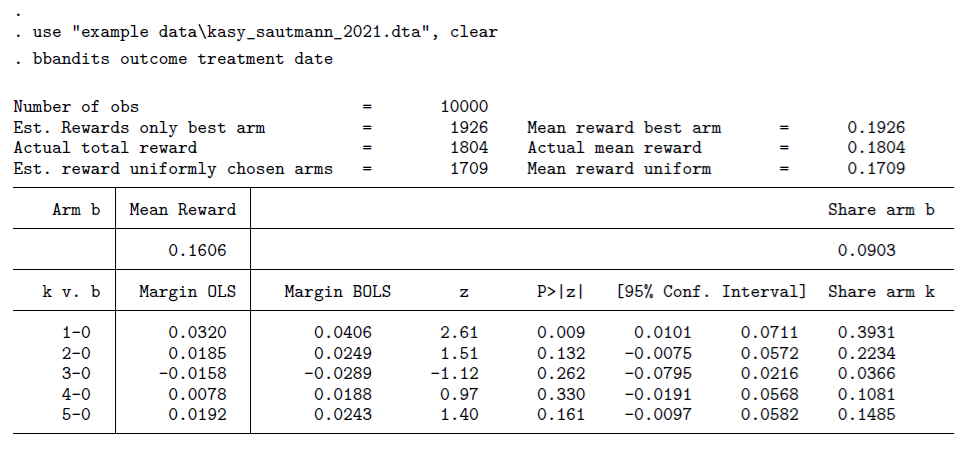
\includegraphics[width=0.9\textwidth]{figures/stlogKasy2021.png}}
\end{center}
\vspace*{-2.5ex}
\end{figure}

\begin{table}
\tiny
    \centering
    \begin{tabular}{lrrrrrr}
    \toprule
Treatment & 0 & 1 & 2 & 3 & 4 & 5\\
         \midrule
         SMS& --- & 1h ahead & 24h ahead & --- & 1h ahead & 24h ahead \\
         Call time& 10 am & 10 am & 10 am & 6:30 pm & 6:30 pm & 6:30 pm \\\bottomrule         
    \end{tabular}
 %   \caption{Caption}
    \label{tab:my_label}
\end{table}

\end{frame}

\begin{frame}{Empirical application \citep{Kasy2021}}

\begin{figure}[h]
\begin{center}
{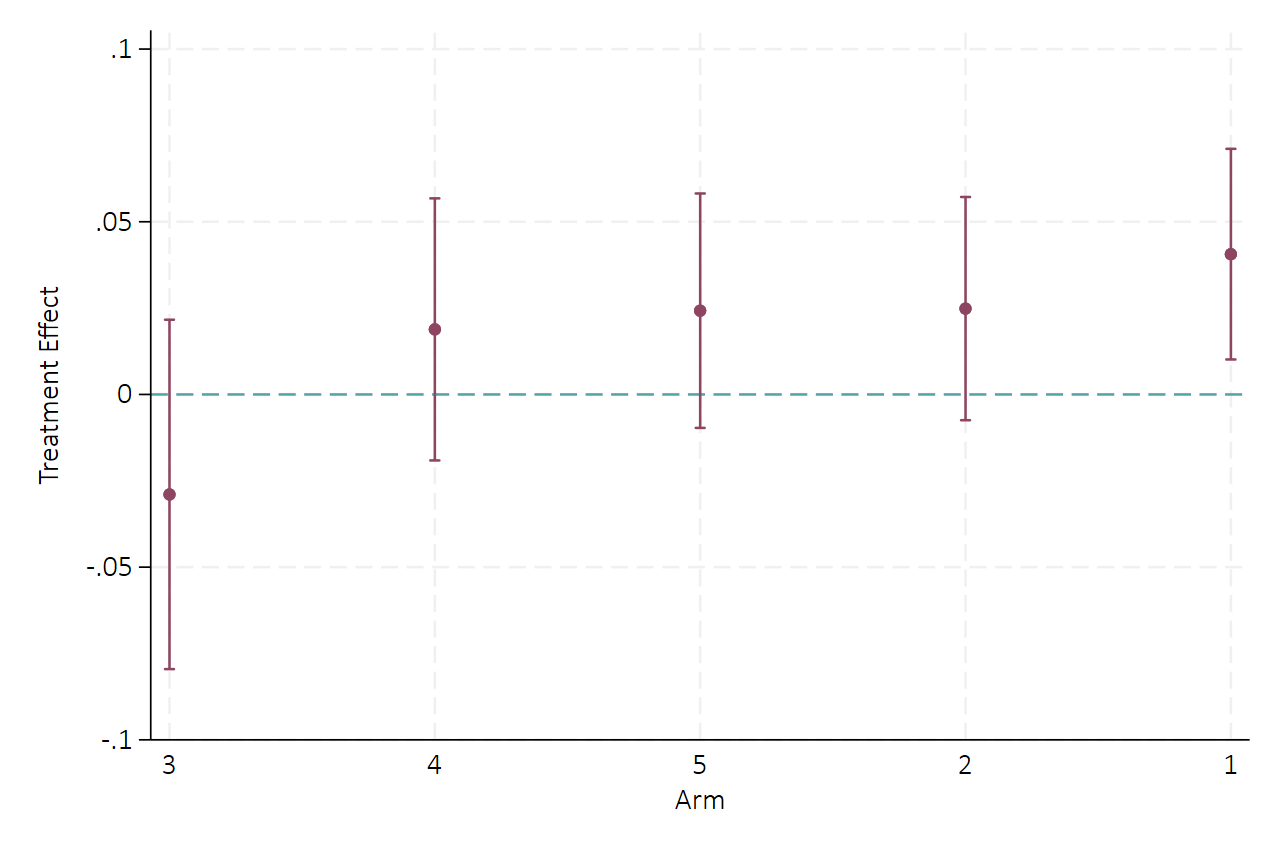
\includegraphics[width=0.9\textwidth]{figures/BOLS_kasy_sautmann.png}}
\end{center}
\vspace*{1ex}
\raggedleft\footnotesize The figure was generated using \texttt{kasy\_sautmann\_2021.dta} and running\\  \href{https://rostam-afschar.de/bbandits/bbandits.htm}{\texttt{bbandits outcome treatment date}}
\vspace*{-4.5ex}
\end{figure}

\end{frame}

\begin{frame}{Empirical application \citep{Kasy2021}}


\begin{figure}[h]
\begin{center}
	\begin{subfigure}[t]{0.49\textwidth}
{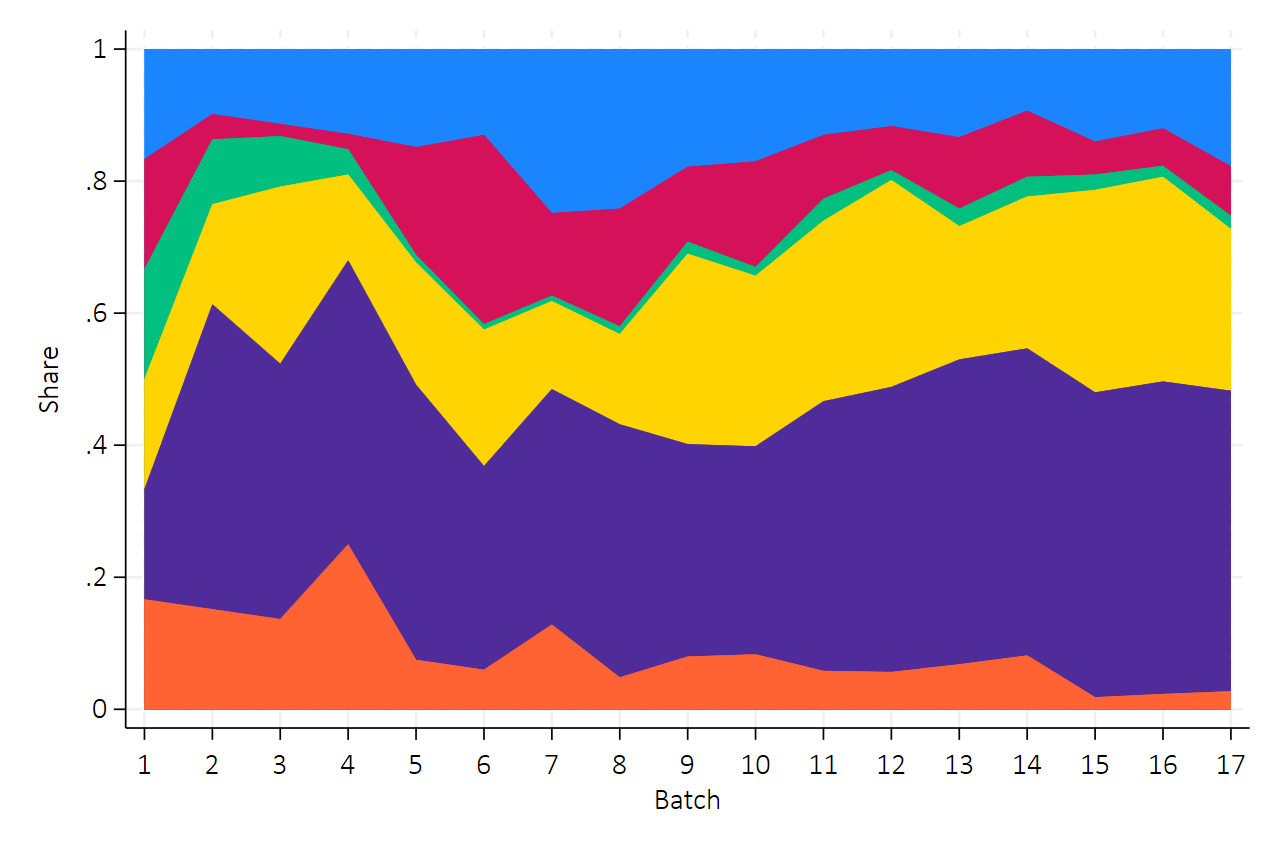
\includegraphics[width=1\textwidth]{figures/StackedShareArmSelected_kasy_sautmann.png}}
            \caption{Batchwise shares}
           \label{fig:Batchwise shares Kasy}		
  \end{subfigure}%
	\begin{subfigure}[t]{0.49\textwidth}
{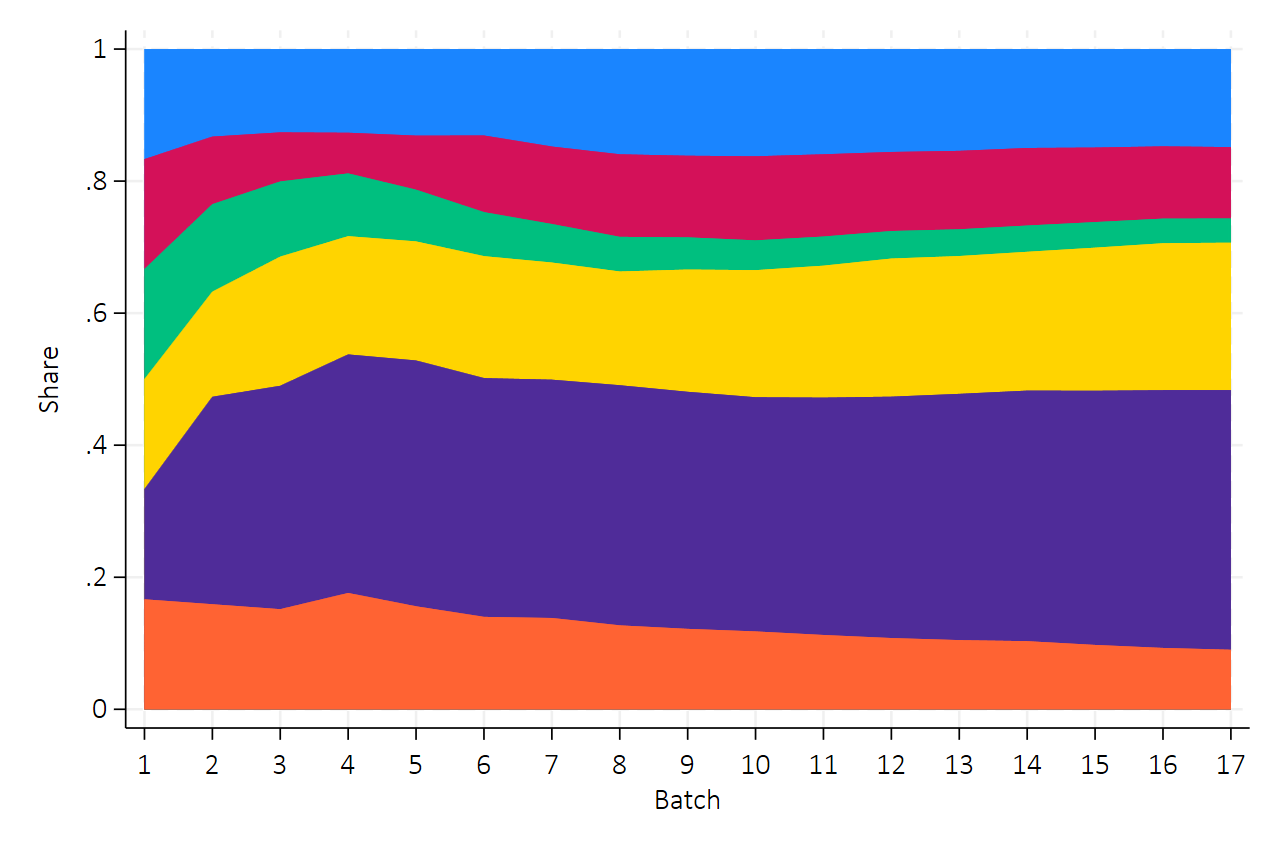
\includegraphics[width=1\textwidth]{figures/CumSharesByBatch_kasy_sautmann.png}}
          \caption{Cumulative shares}
           \label{fig:Cumulative shares Kasy}	
  \end{subfigure}   
\end{center}
\vspace*{1ex}
\raggedleft\footnotesize The figure was generated using \texttt{kasy\_sautmann\_2021.dta} and running\\  \href{https://rostam-afschar.de/bbandits/bbandits.htm}{\texttt{bbandits outcome treatment date}}
\vspace*{-4.5ex}
\end{figure}

\end{frame}

\begin{frame}{Empirical application \citep{Kasy2021}}
\renewcommand{\baselinestretch}{1}
\textcolor{BrewerRed}{Takeaways}\\
\textbf{Clear best and worst arms}
\begin{itemize}
    \item Best: Calling farmers at 10 am after a message an hour ahead
    \item Worst: Calling at 6:30 pm without a text message alert
\end{itemize}
\textbf{Improvement of success rate}
\begin{itemize}
    \item 18.04\% success rates within the experiment
    \item 17.15\% success rate with equal assignment
\end{itemize}


\end{frame}


%
%\begin{frame}{Empirical application \small\citep{Gaul2024}}
%\textbf{32 invitation messages for business survey}
%\renewcommand{\baselinestretch}{1}
%
%\begin{itemize}
    %\item \cite{Gaul2024} designed an experiment using \emph{Thompson sampling} to support the German Business Panel (GBP)
    %\item Aim is to select among a variety of different invitation messages to survey firm decision makers in Germany
%\item The GBP is a web-based survey study of firm decision makers in Germany that invites participants each work day\\ (see \cite{Bischof2024, Hack2024})
%\item The outcome (reward) is a binary variable for the start of the survey:
%\begin{itemize}
    %\item = 1 if email invitation recipient started the survey
    %\item = 0 otherwise
%\end{itemize}
%
%\end{itemize}
%
%\end{frame}
%
%\begin{frame}{Empirical application \small\citep{Gaul2024}}
%
%\begin{minipage}[c]{1\textwidth}
%\resizebox{1\textwidth}{!}{
%\Tree[.\text{Invitation Message Treatments} [.\text{Personalization} [.\text{Firm name P1} ] [.\text{No firm name P0} ]] [.\text{Authority} [.\text{Titles A1} ] [.\text{No Titles A0} ]] [.\text{URL Position} [.\text{Top U1} ] [.\text{Bottom U0} ]] [.\text{Data Protection} [.\text{Paragraph D1} ] [.\text{Sentence D0} ] ] [.\text{Message Frame} [.\text{Plea M1} ] [.\text{Offer M0} ]  ]]
%}
%\end{minipage}
%\vspace{1.5ex}
%\renewcommand{\baselinestretch}{1}
%\begin{itemize}
%\item Five components of invitation letters and their full interactions\\
%$\rightarrow$\quad$2^5=32$ treatments
%\begin{itemize}
    %\item \textbf{personalization} by mentioning or not mentioning the firm name
    %\item \textbf{authority} of the sender by listing the official full academic titles along with the senders' names or their names only
    %\item \textbf{URL position} to start the survey at the top or bottom of the invitation
    %\item \textbf{data protection} in a separate paragraph with two strongly phrased sentences or in a single sentence
    %\item \textbf{message frame} by including phrases that plea for support in the survey's cause or to simply offer to participate
%\end{itemize}
%\end{itemize}
%
%\end{frame}
%
%
%\begin{frame}{Empirical application \small\citep{Gaul2024}}
%\renewcommand{\baselinestretch}{1}
%\begin{itemize}
%
%\item 11,000 randomly selected contacts from firms in Germany
%\item Assigned to each of 15 batches from a list of 176,000 contacts
%\item Each batch corresponds to a week between\\ August 16, 2022 and November 25, 2022
%\item First four batches used fixed and balanced burn-in phase\\ with treatment probability $1/32$
%\item From batch 5, Thompson assignment rule for each consecutive batch
%\end{itemize}
%
%\end{frame}
%
%\begin{frame}{Empirical application \small\citep{Gaul2024}}
%
%\begin{figure}[h]
%\begin{center}
%{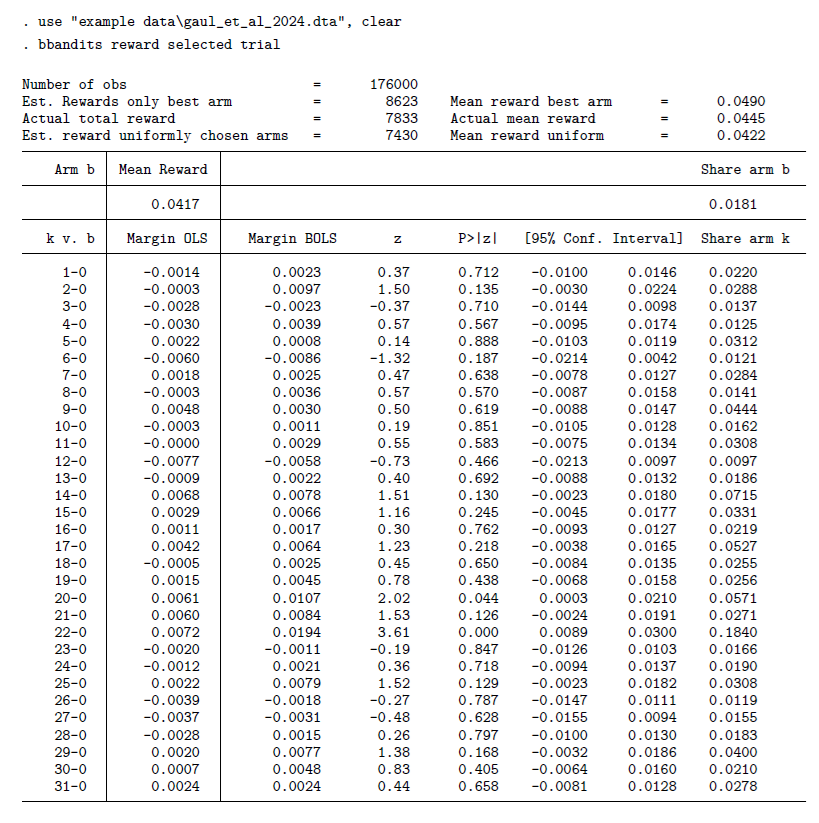
\includegraphics[width=0.7\textwidth]{figures/stlogGaul2024.png}}
%\end{center}
%\vspace*{-4.5ex}
%\end{figure}
%\end{frame}
%
%\begin{frame}{Empirical application \small\citep{Gaul2024}}
%
%\begin{figure}[h]
%\begin{center}
%{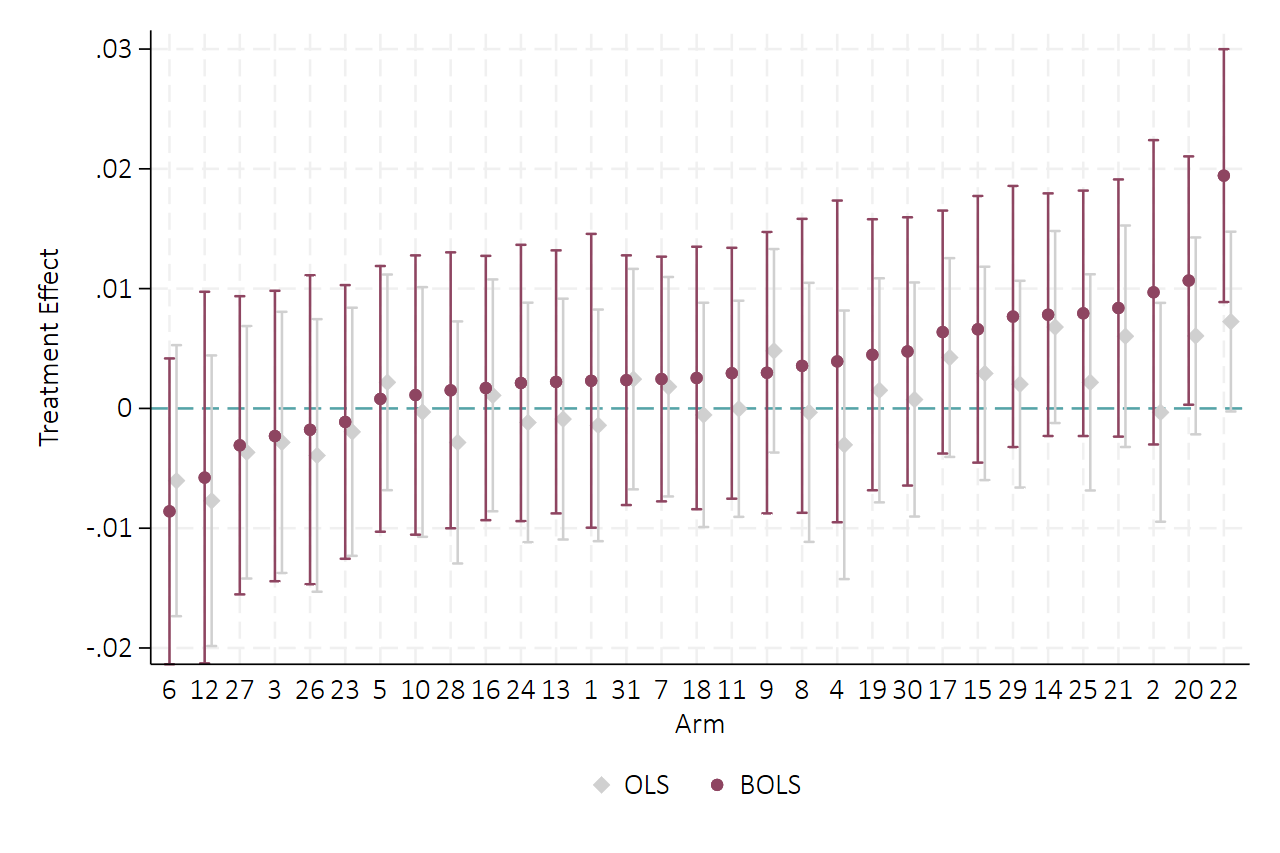
\includegraphics[width=0.9\textwidth]{figures/OLS_gaul_et_al.png}}
%\end{center}
%\vspace*{1ex}
%\raggedleft\footnotesize The figure was generated using \texttt{gaul\_et\_al\_2024.dta} and running\\  \href{https://rostam-afschar.de/bbandits/bbandits.htm}{\texttt{bbandits reward selected trial}}
%\vspace*{-4.5ex}
%\end{figure}
%
%\end{frame}
%
%
%
%
%\begin{frame}{Empirical application \small\citep{Gaul2024}}
%
%
%\begin{figure}[h]
%\begin{center}
	%\begin{subfigure}[t]{0.49\textwidth}
%{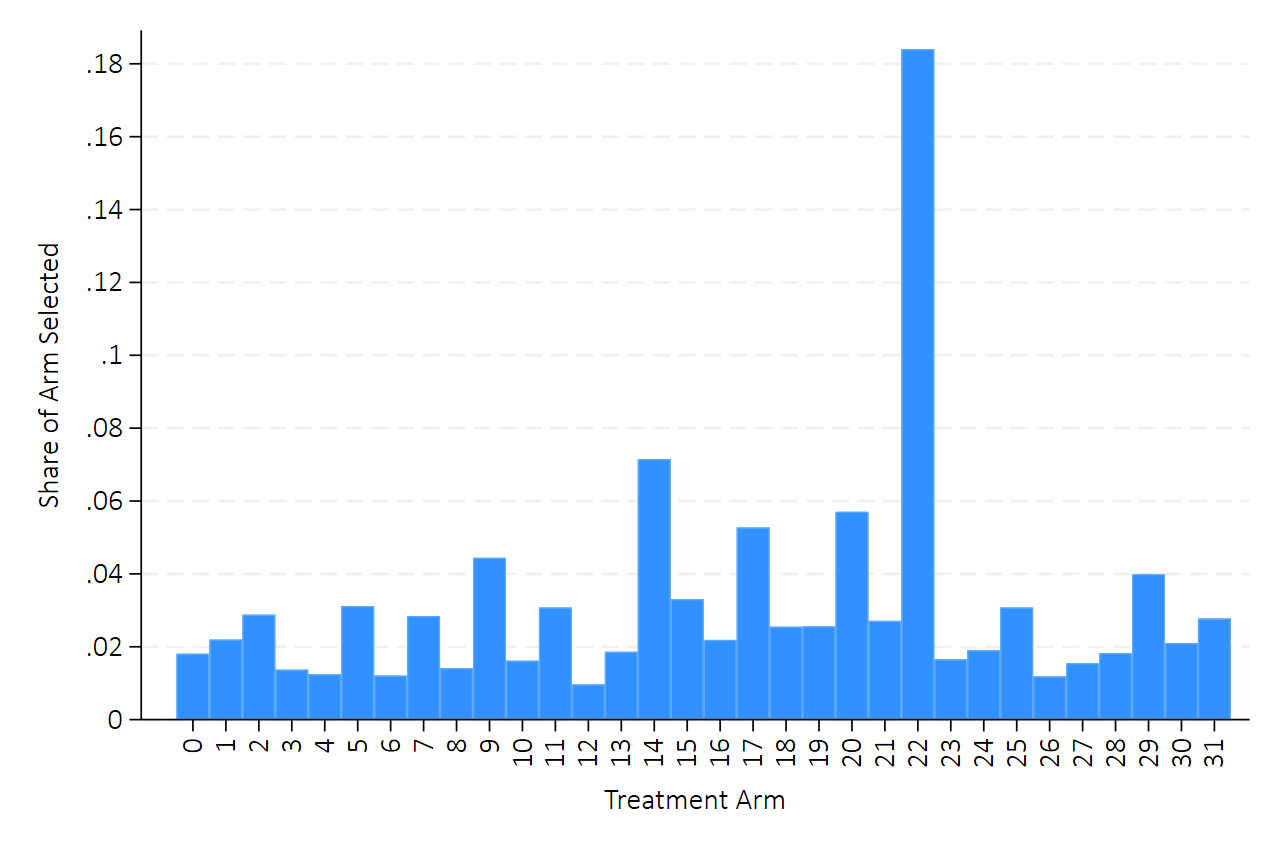
\includegraphics[width=1\textwidth]{figures/ShareArmSelected_gaul_et_al.png}}
           %\caption{Total frequency of treatment assignment}
           %\label{fig:Empirical distribution of standardized OLS estimator for the margin}	
  %\end{subfigure}%
	%\begin{subfigure}[t]{0.49\textwidth}
%{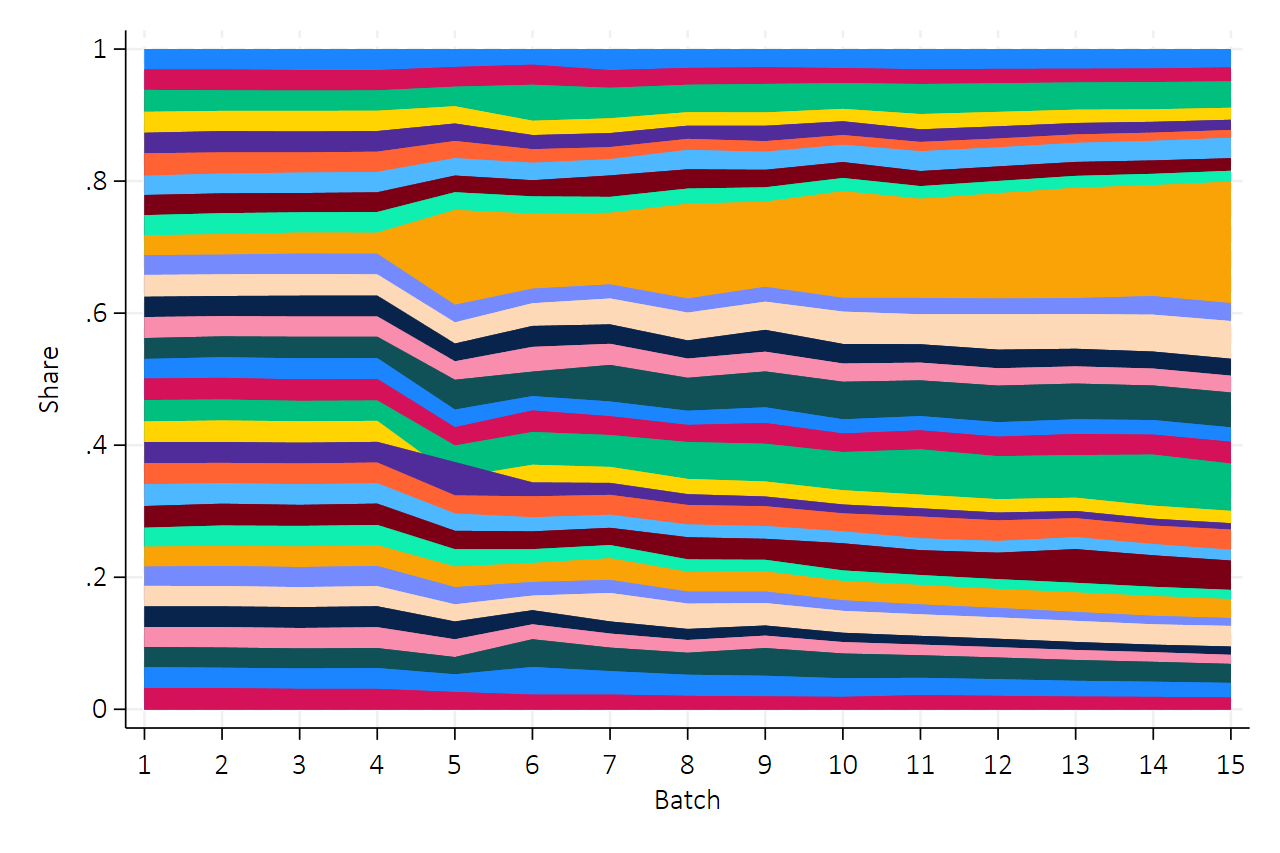
\includegraphics[width=1\textwidth]{figures/CumSharesByBatch_gaul_et_al.png}}
           %\caption{Cumulative shares of arms played}
           %\label{fig:Empirical distribution of standardized BOLS estimator for the margin}	
  %\end{subfigure}   
%\end{center}
%\vspace*{1ex}
%\raggedleft\footnotesize The figure was generated using \texttt{gaul\_et\_al\_2024.dta} and running\\  \href{https://rostam-afschar.de/bbandits/bbandits.htm}{\texttt{bbandits reward selected trial}}
%\vspace*{-4.5ex}
%\end{figure}
%
%\end{frame}
%
%\begin{frame}{Empirical application \small\citep{Gaul2024}}
%\renewcommand{\baselinestretch}{1}
%\textcolor{BrewerRed}{Takeaways}\\
%\textbf{Clear best and worst arms}
%\begin{itemize}
    %\item Using personalization, authority, and pleading for support has greatest success\\[2ex]
%
%\end{itemize}
%\textbf{Interaction effects important, too}\\[2ex]
 %More results in the paper...
%
%\end{frame}
%
%
%
%
%
%\begin{frame}{Monte Carlo Simulations}
%\renewcommand{\baselinestretch}{1}
%\begin{itemize}
    %\item \href{https://youtu.be/x-u2a8GKs-s?si=effdgWoBdCNrC38w}{\textcolor{BrewerRed}{\textit{Click to watch}}: OLS fails normality when margin is small}
    %\item \href{https://youtu.be/YuZi-xHwpQ0?si=C3HbfKu_h-q5_bU5}{\textcolor{BrewerRed}{\textit{Click to watch}}: BOLS normal even when margin is small}
    %\item Run own simulations with\\[1ex] \footnotesize  \href{https://rostam-afschar.de/bbandits/bbandits.htm}{\texttt{bbandit\_sim  0.5 0.4 0.3, size(200) batch(10) clipping(0.1) Thompson plot\_Thompson}}
%\end{itemize}
%
%\end{frame}
%
%
%
%
%\begin{frame}{Best Practices}
%\renewcommand{\baselinestretch}{1}
%
%\begin{itemize}
    %\item Report OLS and BOLS
    %\item BOLS inference in the small margin case \textbf{correct} but...
    %\item OLS inference in the large margin case \textbf{more precise}
    %\item Check batch-wise OLS estimates
    %\item \textbf{At least 50 observations} per batch and arm
    %\item From \textit{statistical testing} perspective:\\ \textbf{more observations} per batch and arm better
    %\item from \textit{regret optimization} perspective\\
    %\textbf{fewer observations} and thus fails are better
    %\item use \textbf{ \href{https://rostam-afschar.de/bbandits/bbandits.htm}{bbandits}} to simulate, visualize, and analyse bandit experiments
%\end{itemize}
%\end{frame}
%
%
%




\begin{frame}[t,allowframebreaks
]%\nocite{*}
\frametitle{References}
\small
\bibliography{bib}
\end{frame}
\section{Takeaways}
{
\setbeamercolor{background canvas}{bg=BrewerBlue}
\begin{frame}
\centering
\Huge
\textcolor{white}{Takeaways}
\thispagestyle{empty}
\end{frame}
}

\begin{frame}{How to run Batched Bandit Experiments?}


\begin{itemize}
    \item Bandits may improve learning and exploitation
    \item There is a push to use more bandits in real experiments in economics, biostats, health, psychology, political science \citep{Offer2021}, \ldots\\ and survey research methods!
    \item need for valid inference to support conclusions
    \begin{itemize}
        \item bandits break inference
        \item researchers want valid confidence intervals
    \end{itemize}
\item \textbf{\textcolor{BrewerRed}{Batched bandit} inference \href{https://rostam-afschar.de/bbandits/bbandits.htm}{(download BBandits)}} 
\begin{itemize}
		\item \citep{Kemper2025}
    \item BOLS allows valid statistical inference \& correct coverage for batched bandits
\end{itemize}
\end{itemize}
\end{frame}

\end{document}
